\documentclass{statsoc}


%======================================================%
%-----------------------------------------------------------------------------------------------%
%****************************************************************************%
%++++++++++++++++++++++++++++++++++++++++++++++++++++++%
%~~~~~~~~~~~~~~~~~~~~~~~~~~~~~~~~~~~~~~~~~~~~~~~~~~~~~~%
%  My Packages and Commands %

%\usepackage{geometry}
\usepackage{fullpage}
%\usepackage{setspace}
%\usepackage[left=1in,top=1in,right=1in]{geometry}
%\pdfpagewidth 8.5in
%\pdfpageheight 11in 


% BIBLIOGRAPHY
\usepackage[authoryear]{natbib}
\bibpunct{(}{)}{;}{a}{}{,}
\linespread{1.5}

\long\def\symbolfootnote[#1]#2{\begingroup%
\def\thefootnote{\fnsymbol{footnote}}\footnote[#1]{#2}\endgroup}


\usepackage{amssymb, amsmath, blindtext, enumitem}
\usepackage{graphicx}
\usepackage{longtable}
\usepackage{dsfont}


\usepackage{listings}


%============================================
%============================================
%My New Commands
%============================================
\newcommand{\balpha}{\mbox{\boldmath $\alpha$} }
\newcommand{\bbeta}{\mbox{\boldmath $\beta$} }
\newcommand{\bdelta}{\mbox{\boldmath $\delta$} }
\newcommand{\bepsilon}{\mbox{\boldmath $\epsilon$} }
\newcommand{\bgamma}{\mbox{\boldmath $\gamma$} }
\newcommand{\blambda}{\mbox{\boldmath $\lambda$} }
\newcommand{\bmu}{\mbox{\boldmath $\mu$} }
\newcommand{\bnu}{\mbox{\boldmath $\nu$} }
\newcommand{\bomega}{\mbox{\boldmath $\omega$} }
\newcommand{\bphi}{\mbox{\boldmath $\phi$} }
\newcommand{\bpsi}{\mbox{\boldmath $\psi$} }
\newcommand{\brho}{\mbox{\boldmath $\rho$} }
\newcommand{\bsigma}{\mbox{\boldmath $\sigma$} }
\newcommand{\btau}{\mbox{\boldmath $\tau$} }
\newcommand{\btheta}{\mbox{\boldmath $\theta$} }
\newcommand{\bupsilon}{\mbox{\boldmath $\upsilon$} }
\newcommand{\bxi}{\mbox{\boldmath $\xi$} }
\newcommand{\bzeta}{\mbox{\boldmath $\zeta$} }
\newcommand{\bDelta}{\mbox{\boldmath $\Delta$} }
\newcommand{\bGamma}{\mbox{\boldmath $\Gamma$} }
\newcommand{\bLambda}{\mbox{\boldmath $\Lambda$} }
\newcommand{\bPhi}{\mbox{\boldmath $\Phi$} }
\newcommand{\bSigma}{\mbox{\boldmath $\Sigma$} }
\newcommand{\bTheta}{\mbox{\boldmath $\Theta$} }

\newcommand{\bfa}{\mbox{\bf a} }
\newcommand{\bfb}{\mbox{\bf b} }
\newcommand{\bfc}{\mbox{\bf c} }
\newcommand{\bfd}{\mbox{\bf d} }
\newcommand{\bfe}{\mbox{\bf e} }
\newcommand{\bff}{\mbox{\bf f} }
\newcommand{\bfg}{\mbox{\bf g} }
\newcommand{\bfh}{\mbox{\bf h} }
\newcommand{\bfi}{\mbox{\bf i} }
\newcommand{\bfj}{\mbox{\bf j} }
\newcommand{\bfk}{\mbox{\bf k} }
\newcommand{\bfl}{\mbox{\bf l} }
\newcommand{\bfm}{\mbox{\bf m} }
\newcommand{\bfn}{\mbox{\bf n} }
\newcommand{\bfo}{\mbox{\bf o} }
\newcommand{\bfp}{\mbox{\bf p} }
\newcommand{\bfq}{\mbox{\bf q} }
\newcommand{\bfr}{\mbox{\bf r} }
\newcommand{\bfs}{\mbox{\bf s} }
\newcommand{\bft}{\mbox{\bf t} }
\newcommand{\bfu}{\mbox{\bf u} }
\newcommand{\bfv}{\mbox{\bf v} }
\newcommand{\bfw}{\mbox{\bf w} }
\newcommand{\bfx}{\mbox{\bf x} }
\newcommand{\bfy}{\mbox{\bf y} }
\newcommand{\bfz}{\mbox{\bf z} }
\newcommand{\bfA}{\mbox{\bf A} }
\newcommand{\bfB}{\mbox{\bf B} }
\newcommand{\bfC}{\mbox{\bf C} }
\newcommand{\bfD}{\mbox{\bf D} }
\newcommand{\bfE}{\mbox{\bf E} }
\newcommand{\bfF}{\mbox{\bf F} }
\newcommand{\bfG}{\mbox{\bf G} }
\newcommand{\bfH}{\mbox{\bf H} }
\newcommand{\bfI}{\mbox{\bf I} }
\newcommand{\bfJ}{\mbox{\bf J} }
\newcommand{\bfK}{\mbox{\bf K} }
\newcommand{\bfL}{\mbox{\bf L} }
\newcommand{\bfM}{\mbox{\bf M} }
\newcommand{\bfN}{\mbox{\bf N} }
\newcommand{\bfO}{\mbox{\bf O} }
\newcommand{\bfP}{\mbox{\bf P} }
\newcommand{\bfQ}{\mbox{\bf Q} }
\newcommand{\bfR}{\mbox{\bf R} }
\newcommand{\bfS}{\mbox{\bf S} }
\newcommand{\bfT}{\mbox{\bf T} }
\newcommand{\bfU}{\mbox{\bf U} }
\newcommand{\bfV}{\mbox{\bf V} }
\newcommand{\bfW}{\mbox{\bf W} }
\newcommand{\bfX}{\mbox{\bf X} }
\newcommand{\bfY}{\mbox{\bf Y} }
\newcommand{\bfZ}{\mbox{\bf Z} }

\newcommand{\calA}{{\cal A}}
\newcommand{\calB}{{\cal B}}
\newcommand{\calC}{{\cal C}}
\newcommand{\calD}{{\cal D}}
\newcommand{\calE}{{\cal E}}
\newcommand{\calF}{{\cal F}}
\newcommand{\calG}{{\cal G}}
\newcommand{\calH}{{\cal H}}
\newcommand{\calI}{{\cal I}}
\newcommand{\calJ}{{\cal J}}
\newcommand{\calK}{{\cal K}}
\newcommand{\calL}{{\cal L}}
\newcommand{\calM}{{\cal M}}
\newcommand{\calN}{{\cal N}}
\newcommand{\calO}{{\cal O}}
\newcommand{\calP}{{\cal P}}
\newcommand{\calQ}{{\cal Q}}
\newcommand{\calR}{{\cal R}}
\newcommand{\calS}{{\cal S}}
\newcommand{\calT}{{\cal T}}
\newcommand{\calU}{{\cal U}}
\newcommand{\calV}{{\cal V}}
\newcommand{\calW}{{\cal W}}
\newcommand{\calX}{{\cal X}}
\newcommand{\calY}{{\cal Y}}
\newcommand{\calZ}{{\cal Z}}

\renewcommand{\Hat}{\widehat}
\renewcommand{\Bar}{\overline}
\renewcommand{\Tilde}{\widetilde}

\newcommand{\iid}{\stackrel{iid}{\sim}}
\newcommand{\indep}{\overset{ind}{\sim}}
\newcommand{\argmax}{{\mathop{\rm arg\, max}}}
\newcommand{\argmin}{{\mathop{\rm arg\, min}}}
\newcommand{\Frechet}{ \mbox{Fr$\acute{\mbox{e}}$chet} }
\newcommand{\Matern}{ \mbox{Mat$\acute{\mbox{e}}$rn} }

\providecommand{\argmin}[1]{\underset{{#1}}{\rm \ argmin}} 
\providecommand{\argmax}[1]{\underset{{#1}}{\rm \ argmax}} 

\newcommand{\seteq}{\stackrel{set}{\ =\ }}

\newcommand{\bfig}{\begin{figure}}
\newcommand{\efig}{\end{figure}}
\newcommand{\beqx}{\begin{equation*}}
\newcommand{\eeqx}{\end{equation*}}
\newcommand{\beq}{\begin{equation}}
\newcommand{\eeq}{\end{equation}}
\newcommand{\beqa}{\begin{eqnarray}}
\newcommand{\eeqa}{\end{eqnarray}}
\newcommand{\beqax}{\begin{eqnarray*}}
\newcommand{\eeqax}{\end{eqnarray*}}
\newcommand{\beqn}{\begin{dmath}}
\newcommand{\eeqn}{\end{dmath}}
\newcommand{\beqnx}{\begin{dmath*}}
\newcommand{\eeqnx}{\end{dmath*}}

\let\originalleft\left
\let\originalright\right
\renewcommand{\left}{\mathopen{}\mathclose\bgroup\originalleft}
\renewcommand{\right}{\aftergroup\egroup\originalright}

\providecommand{\itbf}[1]{\textit{\textbf{#1}}} 
\providecommand{\abs}[1]{\left\lvert#1\right\rvert} 
\providecommand{\norm}[1]{\left\lVert#1\right\rVert}

\newcommand{\cond}{\,\left\vert\vphantom{}\right.}
\newcommand{\Cond}{\,\Big\vert\vphantom{}\Big.}
\newcommand{\COND}{\,\Bigg\vert\vphantom{}\Bigg.}

\providecommand{\paren}[1]{\left(#1\right)} 
\providecommand{\Paren}[1]{\Big(#1\Big)}
\providecommand{\PAREN}[1]{\bigg(#1\bigg)} 
\providecommand{\bracket}[1]{\left[ #1 \right]} 
\providecommand{\Bracket}[1]{\Big[ #1 \Big]} 
\providecommand{\BRACKET}[1]{\bigg[ #1 \bigg]} 
\providecommand{\curlybrace}[1]{\left\{ #1 \right\}} 
\providecommand{\Curlybrace}[1]{\Big\{ #1 \Big\}} 
\providecommand{\CURLYBRACE}[1]{\bigg\{ #1 \bigg\}} 

\newcommand{\Bern}{\mbox{{\sf Bern}}}
\newcommand{\Bernoulli}{\mbox{{\sf Bernoulli}}}
\newcommand{\Beta}{\mbox{{\sf Beta}}}
\newcommand{\Bin}{\mbox{{\sf Bin}}}
\newcommand{\Binomial}{\mbox{{\sf Binomial}}}
\newcommand{\DE}{\mbox{{\sf DE}}}
\newcommand{\Exponential}{\mbox{{\sf Exponential}}}
\newcommand{\F}{\mbox{{\sf F}}}
\newcommand{\Gam}{\mbox{{\sf Gamma}}}
\newcommand{\GP}{\mbox{{\sf GP}}}
\newcommand{\GPD}{\mbox{{\sf GPD}}}
\newcommand{\Geom}{\mbox{{\sf Geom}}}
\newcommand{\Geometric}{\mbox{{\sf Geometric}}}
\newcommand{\HyperGeom}{\mbox{{\sf HyperGeom}}}
\newcommand{\HyperGeometric}{\mbox{{\sf HyperGeometric}}}
\newcommand{\InverseGam}{\mbox{{\sf InverseGamma}}}
\newcommand{\InvWish}{\mbox{{\sf InvWish}}}
\newcommand{\MVN}{\mbox{{\sf MVN}}}
\newcommand{\NB}{\mbox{{\sf NB}}}
\newcommand{\NegBin}{\mbox{{\sf NegBin}}}
\newcommand{\NegativeBinomial}{\mbox{{\sf NegativeBinomial}}}
\newcommand{\Normal}{\mbox{{\sf Normal}}}
\newcommand{\Pois}{\mbox{{\sf Pois}}}
\newcommand{\Poisson}{\mbox{{\sf Poisson}}}
\newcommand{\Unif}{\mbox{{\sf Unif}}}
\newcommand{\Uniform}{\mbox{{\sf Uniform}}}
\newcommand{\Weibull}{\mbox{{\sf Weibull}}}

\renewcommand{\P}{{\sf P}}
\newcommand{\Prob}{{\sf Prob}}
\newcommand{\median}{{\mathop{\rm median}}}
\newcommand{\E}{\mathsf{E}}
\newcommand{\V}{\mathsf{V}}
\newcommand{\VAR}{\mathsf{VAR}}
\newcommand{\COV}{\mathsf{COV}}

\newcommand{\Ind}{\mathds{1}}
\newcommand{\zerovect}{\mbox{\bf 0}}
\newcommand{\onesvect}{\mbox{\bf 1}}
\providecommand{\real}[1]{\mathbb{#1}}
\newcommand{\Real}{\mathbb{R}}
\newcommand{\ppd}{\mathcal{P}}
\DeclareMathOperator{\logit}{logit}
\DeclareMathOperator{\expit}{expit}
\DeclareMathOperator{\dint}{\displaystyle\int}
\DeclareMathOperator{\dsum}{\displaystyle\sum}

%============================================
%My New Commands
%============================================
%============================================


\newcommand{\bitemize}{\begin{itemize}\setlength{\itemsep}{1pt}\setlength{\parskip}{1pt}}
\newcommand{\eitemize}{\end{itemize}}
\newcommand{\benum}{\begin{enumerate}\setlength{\itemsep}{1pt}\setlength{\parskip}{1pt}}
\newcommand{\eenum}{\end{enumerate}}

%\usepackage{fancyhdr}
%\pagestyle{fancy}

%\lhead{\footnotesize \parbox{11cm}{Custom left-head-note} }
%\cfoot{}
%\lfoot{\footnotesize \parbox{11cm}{}}
%\rfoot{\footnotesize Page \thepage\ }
%\rfoot{\footnotesize Page \thepage\ of \pageref{LastPage}}
%\renewcommand\headheight{24pt}
%\renewcommand\footrulewidth{0.4pt}


\usepackage[colorlinks=false,
          %  pdfborder={0 0 0},
            ]{hyperref}


%  My Packages and Commands %
%======================================================%
%-----------------------------------------------------------------------------------------------%
%****************************************************************************%
%++++++++++++++++++++++++++++++++++++++++++++++++++++++%
%~~~~~~~~~~~~~~~~~~~~~~~~~~~~~~~~~~~~~~~~~~~~~~~~~~~~~~%
%______________________________________________________%






%============================================
%============================================
% PREAMBLE
%============================================
%============================================

\title[Graphical modeling of seabird distributions]{Exploring dependencies of multivariate seabird distributions: Linking graphical models to social network analysis}
\author[Author 1 {\it et al.}]{Matthias Eckardt}
\address{Humboldt-Universit{\"a}t zu Berlin,
Berlin,
 Germany.}
\email{Author@emailaddress.com}
\author{Earvin Balderama}
\address{Loyola University Chicago,
         Chicago, IL,
         USA.}
         




%============================================
%============================================
\IfFileExists{upquote.sty}{\usepackage{upquote}}{}
\begin{document}%\linenumbers
%============================================
%============================================



%============================================
\begin{abstract}
  Graphical modeling of seabird distributions. Simultaneous estimation of conditional spatial interrelation for a subset of $204$ seabird species by means of a spatial dependence graph model (SDGM). Linkage to Social network analysis toolbox to detect the most influential species (in term of importance within the estimated SDGM)  
\end{abstract}

\keywords{Graphical modeling, Species importance, Marked point process, Network centrality measures, Seabird distribution}
%============================================



%============================================
\section{Introduction}
%============================================



Information on the spatial distribution of marine birds is of particular interest to ecologists, environmentalists and policy-makers. 
%Individual species maps conveying the spatial and temporal distribution over the US Mid- and Northeast-Atlantic ocean regions were created by~\cite{Balderama2016} for several sea bird species.  

%Models are usually run on individual species. 
%There is a danger in this, in that it doesn't take into account the dependence structure between species. 
There is a danger in this in that it is generally known that species distributions are not independent.
Maps of the spatial distribution of marine birds undoubtedly have some overlap
%It creates a false sense that a species distribution is independent

Models are usually run on either individual species or all-species-combined data. \cite{Winiarski2014} first categorized species into different taxonomic groups before fitting a separate model to each grouping. \cite{Balderama2016} modeled several species individually and created separate distribution maps for each species. 







In ecology,
Quantifying the spatial dependence structure between bird species and environmental covariates is important. While studies have related the spatial distribution of one species with that of a prey or predator species or of environmental variables acting as proxies for climate \citep{Goyert2014, Goyert2016}, there has been relatively few studies that investigate and utilize measures of inter-species dependence.

Community models may combine several species, known to have facilitative interactions with each other, into one model \citep{Goyert2016, Sollmann2016}. However, these models treat the observed data the same way as if the observations belong to the same species, i.e., come from the same distribution.



Studying the degree of interaction between species may help inform ocean planning and develop effective strategies for ecosystem management. Mapping the distribution of rare and endangered avian species is important when planning the placement of offshore wind energy developments. Such rare species are obviously difficult to monitor, so finding a more commonly occurring species that is highly dependent with the rare species has ecological importance.






Ecological data usually contains spatial observations from multiple species of interest. 







The occurrence of a sea bird species in a particular location is affected (either positively or negatively) by the occurrence of other species in the same location. 
Thus, external factors that may cause changes to the distribution of a single species will undoubtedly have an effect on the distribution of other species. 
Determining these associations between different species has been difficult~\citep{Stachowicz2001}, especially when trying to find the associations between many species all at once.
Attempts at modeling between-species interactions are often limited to the bivariate case \citep{Andersen1992, Nightingale2015}. For three or more species, models are usually hindered by computing time due to the estimation of very many interaction parameters \citep{Jalilian2015}. 

At the same time, there is a need for fast and practically applicable methods for analyzing multivariate point patterns, and this is currently a growing but challenging topic for researchers~\citep{Moller2016}.



In this paper, we explore the dependence structure between multiple sea bird species distributions, using the graphical modelling approach of~\cite{Eckardt2016b}. %%%%%%%%%


%There are several advantages with this approach:
Using this approach,
1. A multivariate analysis of sea bird distributions may be useful in determining how one bird species affects the presence of another. 

2. This will help us to categorize observations of unidentified or unknown species to those of identified species.  

Observations labelled as ``unidentified'' are often removed before analyzing data at the species level. Here we include these data and may be able to determine what species they are most likely to be from the resulting network map. 


The sea bird data is described, as a multivariate spatially marked point process, in Section~\ref{Data}. We apply the graphical model to the sea bird data in Section~\ref{Methods} and illustrate some resulting network maps in Section~\ref{Results}. Concluding remarks are given in Section~\ref{Conclusions}.
















%============================================
\section{Data}\label{Data}
%============================================




Data are point locations of marine bird sightings over the Northeast- and Mid-Atlantic coast regions of the United States, as described in \cite{Balderama2016}. The point locations are the longitude and latitude coordinates of the midpoints of transect segments from boat and aerial strip transect surveys between July, 1998 and April, 2014. Out of 90660 total point locations for potential sightings, 53842 have at least one species sighting. Because more than one species may be sighted in any one location, the full data contains 128812 total species-location combinations. Species are labelled by its common name and a corresponding four-letter species code. The full data contains 306 different codes. Some codes signify an unidentified or partially identified species. For example, the word ``unidentified'' may accommodate birds that have been identified to a family but not to a species. In this paper, however, we will use the term ``species'' to refer to different four-letter codes.
For our analysis we consider only 204 (out of 306) species that have been sighted in at least three locations. By this, our analysis covers 53820 locations and 128674 species-location combinations.

A sighting is a recorded observation at least one individual bird. In the context of spatially marked point patterns, each sighting corresponds to one point of a species' point pattern, with the mark of the point being the number of birds observed in that sighting. Table~\ref{tab:species} shows the total number of birds observed and the average mark for the twenty most frequently recorded bird species by common name and species code.
Observed planar point patterns for these twenty most sighted species are shown in Figure~\ref{fig:birds20}.

%\textit{ For our analysis we considered on 128812 locations on marine bird sightings related to 306 different marine birds. Form this data, we preselected a sample of 204 species which have have at least been observed at three locations. By this, our analysis covered 128674 different locations.}


 
\begin{figure}
\centering
\makebox{\includegraphics[scale=0.45]{BirdsTop20.eps}}
      \caption{\label{fig:birds20} Spatial point patterns of the $20$ most frequently observed marine bird species.}
\end{figure} 


%\textbf{Maybe reduce table to most frequent species, eg. top 20 birds}



%latex.default(format.df(latdf, cdec = c(0, 0, 0, 0, 2), na.blank = TRUE),     file = "", longtable = TRUE, rowname = NULL, size = "scriptsize",     caption = "Summary of top 20 most frequently sighted species.",     label = "tab:species")%
\setlongtables{\scriptsize
\begin{longtable}{llrrr}\caption{Summary of top 20 most frequently sighted species.} \tabularnewline
\hline\hline
\multicolumn{1}{c}{Species code}&\multicolumn{1}{c}{Common name}&\multicolumn{1}{c}{total}&\multicolumn{1}{c}{sightings}&\multicolumn{1}{c}{average mark}\tabularnewline
\hline
\endfirsthead\caption[]{\em (continued)} \tabularnewline
\hline
\multicolumn{1}{c}{Species code}&\multicolumn{1}{c}{Common name}&\multicolumn{1}{c}{total}&\multicolumn{1}{c}{sightings}&\multicolumn{1}{c}{average mark}\tabularnewline
\hline
\endhead
\hline
\endfoot
\label{tab:species}
BLSC&Black Scoter&$ 88865$&$ 2444$&$ 36.36$\tabularnewline
COEI&Common Eider&$958282$&$ 4127$&$232.20$\tabularnewline
COLO&Common Loon&$ 17456$&$ 6795$&$  2.57$\tabularnewline
COSH&Cory's Shearwater&$  9434$&$ 2328$&$  4.05$\tabularnewline
COTE&Common Tern&$ 15054$&$ 2212$&$  6.81$\tabularnewline
GBBG&Great Black-backed Gull&$ 26882$&$ 7581$&$  3.55$\tabularnewline
GRSH&Greater Shearwater&$ 64941$&$ 6213$&$ 10.45$\tabularnewline
HERG&Herring gull&$ 55233$&$10990$&$  5.03$\tabularnewline
LAGU&Laughing Gull&$ 12535$&$ 2834$&$  4.42$\tabularnewline
LTDU&Long-tailed Duck&$209151$&$ 5602$&$ 37.34$\tabularnewline
NOGA&Northern Gannet&$ 81759$&$12831$&$  6.37$\tabularnewline
RAZO&Razorbill&$ 17306$&$ 2410$&$  7.18$\tabularnewline
RTLO&Red-throated Loon&$ 16039$&$ 4737$&$  3.39$\tabularnewline
SUSC&Surf Scoter&$106770$&$ 4059$&$ 26.30$\tabularnewline
UNGU&Unidentified Gull&$ 39067$&$ 3976$&$  9.83$\tabularnewline
UNLO&Unidentified Loon&$ 31741$&$ 3962$&$  8.01$\tabularnewline
UNSC&Unidentified Scoter&$546211$&$ 3950$&$138.28$\tabularnewline
UNTE&Unidentified Tern&$ 24232$&$ 2331$&$ 10.40$\tabularnewline
WISP&Wilson's Storm-petrel&$ 40689$&$ 4845$&$  8.40$\tabularnewline
WWSC&White-winged Scoter&$ 33095$&$ 2310$&$ 14.33$\tabularnewline
\hline
\end{longtable}}





While some marine bird species, such as various types of gulls, have been sighted at numerous locations, other species occurred only very rarely. At the same time, as we defined a minimum of at least $50$ marine birds per species as inclusion criteria, this limited number of locations equivalently implies that certain marine bird species appeared in groupings rather than as isolated birds or occurred only in a geographically strictly-limited habitat. An example of such only rarely observed species are black-capped petrels whose $50$ counted sighting have only been recorded at $n=3$ different locations. This reflects our expectations, as black-capped petrels have been classified as endangered species by the IUCN Red List of Threatened Species. Discovering the relevant subset of species whose spatial occurrence is linked to the spatial pattern of any endangered species  by means of a SDGM might provide new insights into multivariate interdependencies.  These new insights might provide important knowledge for the conservation of endangered species and might assist to understand such phenomena from a global perspective on different natural environments.    



%============================================
\section{Methods}
%============================================

data as multivariate marked spatial point process as defined in \cite{Eckardt2016b}. 

literature on point process
\cite{Chiu2013}, \cite{Illian2008} and \cite{StoyanStoyan1994}.
For a comprehensive treatment of various models and statistics for marks and points we refer the interested reader to \cite{Illian2008}, \cite{Baddeley2010} and \cite{WiegandMoloney2013}

\begin{itemize}
\item We estimate the conditional spatial dependence structure between different seabird species
\item that is, structural dependence between two patterns conditional on all remaining patterns
\item so not interrelation between points $i$ and $j$, but interrelations between components $i$ and $j$ where $i$ and $j$ are sets of points within a bounded planar region.
\item edges express the partial (pairwise) interrelation between two species conditional on al remaining species
\item we omit to implement a formal test statistic as we assume that dependence might vary between species
\item we set a threshold indicating weak/ intermediate partial effects
\item we combine spatial dependence graph model with importance tools of social network analysis
\item info can provide important insides for species conservation
\item eg which are the most important species in the overall graph
\end{itemize}

Primary idea by \cite{Eckardt2016}, extension to multivariate spp with quantitative marks by \cite{Eckardt2016b}

Analysis was carried out using the \texttt{sdgm} R package of \cite{Eckardt2016a}.

For an intense description of different aspects of network analysis we refer the interested reader to \cite{Carrington2005}, \cite{Kolaczyk:2009} and \cite{Goldenberg:EtAl:2010}.


Although graphical modelling and network analysis are two distinct fields and are in general treated separately, the conjunction of both fields could offer additional benefits for the analysis of multivariate spatial data.  Especially for the analysis of high-dimensional spatial data one might be interested in the structural importance of a distinct node in a given SDGM. That is, how substantial is the impact of a certain node on the observed network structure. Queries of this type are covered by centrality measures which aim to value the importance of a distinct  node in the network. Although a rich methodological toolbox for the structural analysis of (social) network data exist, we only  we considered four different centrality measures: the degree, the closeness, the betweenness and the eigenvector centrality (cf. \cite{Borgatti2006, Freeman1979, Newman2004}). Although these measure are similar in spirit, they are different in detail and each of these three centrality measures formalizes a different concept of importance from a (social) network  perspective.

\textbf{meaning}
 Betweenness centrality measures the number of shortest paths
going through a specific vertex

Closeness is the mean geodesic distance between a given node and
 all other nodes with paths from the given node to the other
 node. This is close to being the mean shortest path, but 
geodesic distances give higher values for more central nodes.

 Eigenvector centrality gives greater weight to a node the more 
 it is connected to other highly connected nodes. A node
 connected to five high-scoring nodes will have higher 
 eigenvector centrality than a node connected to five low-scoring
 nodes. Thus, it is often interpreted as measuring a node's
 network 



For our analysis we estimated all marked auto- and cross-spectral densities for all $204$ species nonparametrically using a discrete Fourier transform of the demeaned mark values. Form this, we computed separate spectra density matrices of dimension $204 \times 204$ for all frequencies. To obtain the mSDGM, we finally inverted and rescaled each matrix such that an edge in the mSDGM is equivalent to non-vanishing absolute rescaled marked inverse spectral value in at least one frequency. To capture variation in strength of spatial interdependencies in our data, we choose two arbitrary thresholds $\alpha$ for the edges below of which we assume two patterns as conditional uncorrelated. That is, as our data contains a wide range of differently-sized of marine bird species we assume a variation in strength of spatial interrelations between different types of trees. A similar idea has been proposed by \cite{GatherImhoffFried2002} with respect to intensive care monitoring.


computed two different mSDGMs by using two thresholds $\alpha=0.3$ and $\alpha=0.6$. 




%============================================
\section{Results}
%============================================

$\star$ in general: important for species conservation: e.g. black-capped petrels only linked to unidentified goldeneyes, both listed as threatened species by IUCN. 


$\star$ most important species by means of the degree centrality are unidentified alcids, Arctic terns, barn swallows, red phalaropes, dovekies, buffleheads, brown pelicans, unidentified mergansers and great black-backed gulls.


$\star$ these species are most often linked to alternative species (no. adjacent species)


$\star$ buffleheads, royal terns, unidentified alcids, Arctic terns, common murres, barn swallows, greater shearwaters, manx shearwaters, Bonaparte's gulls and Northern gannets are the most important species by means of the betweenness centrality.


$\star$ these species are most often intermediate species, that is most links from a to b path through these species

For our first mSDGM, we considered a threshold $\alpha=0.3$ which we interpret as a conditional interrelation of weak effect size. For this, we treated all values of the empirical absolute rescaled marked inverse spectra below $\alpha=0.3$ as zero. The resulting mSDGM  is depicted in Figure \ref{fig:g30}.


\begin{figure}
\centering
\makebox{\includegraphics[scale=0.5]{rawg30.eps}}
      \caption{\label{fig:g30} Marked spatial dependence graph model for the $204$ different marine bird species, and bird counts as quantitative mark for a threshold level of $\alpha=0.3$.}
\end{figure} 



This SDGM consisted of two $4$-node subgraphs, a $6$- node subgraph and a $153$-node subgraph and of 3400 edges. Besides, we also found $37$ isolated species (AMCO, AMPI, AMRE, BAOR, BLPW, BRAN, BTBW, BUPE, COYE, FEPE, GCKI, GRCA, LESC, LISH, MABO, MAWA, MERL, NOFL, NOHA NOTE, NOWA, PEFA, RBTR, RCKI, RTHU, RUBL, SAVS, SNBU, SPAR, Surf Scoter, UNHU, UNPT, UNTB, USAN, WTSP, YBCH, YWAR). These findings imply that non of the $37$ species are interrelated to any other species taken into account at threshold $\alpha=.3$. This could mean that the isolated nodes tend to represent species whose marked point patterns are different from all remaining marked point patterns taken into account. This is an interesting result as the isolated nodes are related to both frequent and endangered species and also differently-sized types of marine birds. One reason for this could be due to our sample scheme. We restricted the dataset to a subset of $204$ different marine bird species, so while there probably are interrelations of this $37$ aerial species to alternative types of birds, the alternative birds did not appear in our subsample. However, the global interrelations within coastal habitat are very complex and are still not completely understood.


Although several findings could be discussed in detail, we only considered structural interdependies for the marked patterns of Roseate Tern, Least Tern and the endangered species Black-capped Petrel, GBHE, YCNH and SAVS.

We begin our discussion with the structural interrelations for Roseate Tern and Least Tern. While we found $62$ conditionally interrelated marked patterns for Roseate Tern, we only observed $10$ interdependent species for Least Tern. For Roseate Tern, these species are Dovekie, AMGO, AMKE, AMOY, AMRO, BBPL, BHCO, BHGU, Red-necked Phalarope, Red Phalarope, BRBO, CHSW, DUNL, EUST, Forster's Tern, SBDO, GRYE, HADU, HOME, LEYE, NOPI, MALL,  Manx Shearwater, PAWA, PEEP, PESA, PISI, RBNU, REDH, RUDU, RUTU, SAGU, SATE, Unidentified Scaup, Pomarine Jaeger, Red-breasted Merganser, Ring-billed Gull, Great or Lesser Black-backed Gull, UCAT, UNBI, UNFR, UNPE, Unidentified Large Alcid , Unidentified Large Gull, Unidentified Merganser, Unidentified Small Tern, BANS, WHIM, GREG, MODO, Unidentified Storm-petrel, WIPH, WODU, YCNH, YRWA, BRSP, BLKI, Black-capped Petrel,   BonapArctic Tern's Gull, BRNO, Common Goldeneye and Dark Scoter. 
For Least Tern we have edges to   Common Murre, Barn Swallow, Arctic Tern, Unidentified Cormorant, Unidentified Shorebird, Unidentified Diving/Sea Duck, South Polar Skua, Unidentified Grebe, Black Guillemotand, Parasitic Jaeger.
 


For GBHE we observed $74$ direct interrelations to alternative marine birds, namely AMGO, AMKE, AMOY, AMRO, BBPL, BHCO, BHGU, GRCO, BRBO, CATE, CHSW, COME, DEJU, DUNL, EUST,  GADW, GRHE, SBDO, GRYE, HADU, HOME, LESA, LEYE, 
LIGU, NOPI, HEPE, ICGU, LTJA, MALL, OSPR,  PAWA, PEEP, PESA, PISI, PUMA, PUSA, RBNU, REDH,  RUDU, RUTU, RWBL, SAGU, SAND, SATE, SEPL,
 SESA, SOSP, SPSA, TRES, UCAT, ULSB, UNEI, UNFR, UNPE, BANS, UNWA, MYWA, WFSP, WHIM, GLGU,  GOME, GREG, MODO, BRTE, WILL, WIPH, WODU, YCNH, YRWA, UCRT, BLTE, BRNO, CANG, and, lastly, AWPE. \textbf{These birds are .....}.  
 
Similarly, focussing on the interrelation which are present for YCNH, we found $79$ links. These interdependent species are  AWPE, Common Loon, Dovekie, Great Black-backed Gull, AMGO, AMKE, AMOY, AMRO, BBPL, BHCO, BHGU, Great Shearwater, Roseate Tern, BRBO, CHSW, COME, DEJU, DUNL, EUST, GADW, GRHE, GBHE, SBDO, GRYE,  HADU, HOME, LESA, LEYE, NOPI, ICGU, Laughing Gull, MALL, OSPR, PAWA, PEEP, PESA, PISI, PUSA, RBNU
 REDH, RUDU, RUTU, RWBL, SAGU, SATE, Unidentified Scaup, SEPL, SESA, SOSP, Pomarine Jaeger, Ring-billed Gull, SPSA, TRES, UCAT  ULSB, UNBI, UNEI, UNFR, UNPE, Unidentified Large Gull, Unidentified Merganser, Unidentified Small Tern, BANS, WFSP, WHIM, GLGU, GOME, GREG, MODO, WILL, WIPH, WODU, YRWA, UCRT, BLKI, Black-capped Petrel,   BonapArctic Tern's Gull, BRNO and CANG.\textbf{These birds are .....}. 
 
For Black-capped Petrel, we found 64 alternative marked point patterns which are directly interrelated to the spatial marked pattern of Black-capped Petrel. These species are 
  Dovekie, AMGO, AMKE, AMOY, AMRO, BBPL, BHCO, BHGU, Red-necked Phalarope, Red Phalarope, Roseate Tern, BRBO, CHSW, DUNL, EUST, Forster's Tern, SBDO, GRYE, HADU, HOME, LEYE, NOPI, Horned Grebe, Laughing Gull, MALL,  Manx Shearwater, PAWA, PESA, PISI, RBNU,  REDH, RUDU, RUTU, SAGU, SATE, Unidentified Scaup, Pomarine Jaeger, Red-breasted Merganser,  Ring-billed Gull, Sooty Shearwater, Great or Lesser Black-backed Gull, UCAT, UNBI, UNFR, UNPE,
 Unidentified Large Alcid , Unidentified Large Gull, Unidentified Merganser, Unidentified Small Tern, BANS, WHIM, GREG, MODO,  Unidentified Storm-petrel, WIPH, WODU, YCNH, YRWA, BRSP, BLKI,
   BonapArctic Tern's Gull, BRNO, Common Goldeneye, and Dark Scoter. \textbf{These birds are .....}. 
 

\textbf{Interestingly, SAVS is isolated in both SDGMs}

These findings imply the presence of complex conditional interdependencies between the marked spatial pattern of GBHF and also YCNH to a wide range of alternative species whereas we found no spatial interdependencies for SAVS to any alternative species taken into account. 


  

As a second model, we also computed a SDGM for a threshold $\alpha=.6$. (we interprete this as interdependencies of intermediate effect size). The resulting mSDGM is depicted in Figure \ref{fig:g60}.

\begin{figure}
\centering
\makebox{\includegraphics[scale=0.5]{rawg60.eps}}
      \caption{\label{fig:g60} Marked spatial dependence graph model for the $204$ different marine bird species, and bird counts as quantitative mark for a threshold level of $\alpha=0.3$.}
\end{figure} 

In this SGDM, we observed two pairs of joined nodes, a $3$-node subgraph, a $4$-node subgraph, a $6$-node subgraph, a $7$-node subgraph, a $8$-node subgraph, a $10$-node subgraph, a $49$-node subgraph and a , a $4$-node subgraph, a $6$-node subgraph, a $71$-node subgraph and $1880$ edges. In addition, we also found $42$ isolated nodes, namely AMCO, AMPI, AMRE, BAOR, BLPW, BRAN, BTBW, BUPE, COYE, FEPE, GCKI, GRCA, Herring Gull, LESC, LISH, MABO, MAFR, MAWA, MERL, NOFL, NOHA, NOTE, NOWA, PEFA, RBTR, RCKI, RTHU, RUBL, SAVS, SNBU, SPAR, Surf Scoter, SWAL, UNDU, UNHU, Unidentified Passerine, UNPT, UNTB, USAN, WTSP, YBCH, YWAR. Again, for the isolated nodes, we concluded that non of marked spatial patterns of these species is conditionally interdependent to any alternative marked pattern taken into account at a threshold $\alpha=.6$.  

As before, we first discuss the spatial interdependencies for Roseate Tern and Least Tern. In contrast to our previous findings, only $13$ edges remain for Roseate Tern at a threshold $\alpha=.6$, namely Red-necked Phalarope, Forster's Tern, Unidentified Scaup, Pomarine Jaeger, Ring-billed Gull, Unidentified Merganser, Unidentified Small Tern, BRSP, BLKI, Black-capped Petrel,   BonapArctic Tern's Gull, Common Goldeneye, and Dark Scoter.

Least Tern is linked to 7 from 204 species, named:
   Common Murre Arctic Tern Unidentified Cormorant Unidentified Diving/Sea Duck South Polar Skua Black GuillemotParasitic Jaeger

\textbf{ .....}

With respect to the marked spatial pattern of GBHE, the neighborhood consisted of $41$ alternative species, namely AWPEBANS, BHCO, BHGU,  BLTE,  CATE, CANG, CHSW, COME, DEJU, DUNL, GLGU, GOME, GRCO, LESA, LIGU, ICGU, LTJA, MALL, MODO, MYWA, OSPR, PAWA, PEEP, PUMA, REDH, RUTU, RWBL, SAND, SEPL, SESA, SOSP, TRES, UNEI, UNFR, UNPE,  UNWA, YRWA, WFSP, WHIM, and WODU.
 
\textbf{...}

For YCNH we detected $52$ interrelated species at a threshold $\alpha=.6$. 
  AMGO, AMKE, AMOY, AMRO, BBPL, BHCO, BHGU, BRBO, CHSW, COME, DUNL, EUST, SBDO, GRYE, HADU, HOME, LESA, LEYE, NOPI, ICGU, MALL, OSPR, PAWA, PEEP, PESA, PISI, RBNU, REDH, RUDU, RUTU, RWBL, SAGU, SATE, SEPL, SESA, SOSP,
 UCAT, UNEI, UNFR, UNPE, BANS, WFSP, WHIM, GOME, GREG,
 MODO, WIPH, WODU, YRWA, BRNO, CANG and AWPE. 
 
\textbf{...}

Similarly, only $13$ conditional interdependencies remained with respect to the marked pattern of  Black-capped Petrelfor a threshold $\alpha=.6$ including the marked point patterns of Red-necked Phalarope, Roseate Tern, Forster's Tern, Unidentified Scaup, Pomarine Jaeger, Ring-billed Gull, Unidentified Merganser, Unidentified Small Tern, BRSP, BLKI,   BonapArctic Tern's Gull, Common Goldeneye and also Dark Scoter.


  





To detect the most influential species within our data, we compute 4 different centrality measures (listed Table \ref{tab:centrality:measures}). The results for the threshold $\alpha=.3$ are listed below, isolated species excluded.

\begin{table}
\caption{\label{tab:centrality:measures}Centrality measures for SDGM for threshold $\alpha=.3$. Isolated nodes excluded.}
\centering
\fbox{%
\begin{tabular}{*{5}{c}}
\em code &\em degree &\em betweenness &\em closeness &\em eigen\\
\hline
MALL  &  $80$  &  $80.370354$  &  $9.37E-05$  &  $1.000000e+00$\\
BANS  &  $80$  &  $80.370354$  &  $9.37E-05$  &  $1.000000e+00$\\
WHIM  &  $80$  &  $80.370354$  &  $9.37E-05$  &  $1.000000e+00$\\
WODU  &  $80$  &  $80.370354$  &  $9.37E-05$  &  $1.000000e+00$\\
AMKE  &  $79$  &  $64.521344$  &  $9.37E-05$  &  $9.930130e-01$\\
AMRO  &  $79$  &  $64.521344$  &  $9.37E-05$  &  $9.930130e-01$\\
BBPL  &  $79$  &  $64.521344$  &  $9.37E-05$  &  $9.930130e-01$\\
BHCO  &  $79$  &  $74.852463$  &  $9.37E-05$  &  $9.917427e-01$\\
BRBO  &  $79$  &  $64.521344$  &  $9.37E-05$  &  $9.930130e-01$\\
CHSW  &  $79$  &  $64.521344$  &  $9.37E-05$  &  $9.930130e-01$\\
EUST  &  $79$  &  $64.521344$  &  $9.37E-05$  &  $9.930130e-01$\\
SBDO  &  $79$  &  $64.521344$  &  $9.37E-05$  &  $9.930130e-01$\\
GRYE  &  $79$  &  $64.521344$  &  $9.37E-05$  &  $9.930130e-01$\\
HADU  &  $79$  &  $64.521344$  &  $9.37E-05$  &  $9.930130e-01$\\
HOME  &  $79$  &  $64.521344$  &  $9.37E-05$  &  $9.930130e-01$\\
LEYE  &  $79$  &  $64.521344$  &  $9.37E-05$  &  $9.930130e-01$\\
NOPI  &  $79$  &  $64.521344$  &  $9.37E-05$  &  $9.930130e-01$\\
PAWA  &  $79$  &  $64.521344$  &  $9.37E-05$  &  $9.930130e-01$\\
PESA  &  $79$  &  $64.521344$  &  $9.37E-05$  &  $9.930130e-01$\\
PISI  &  $79$  &  $64.521344$  &  $9.37E-05$  &  $9.930130e-01$\\
RBNU  &  $79$  &  $64.521344$  &  $9.37E-05$  &  $9.930130e-01$\\
RUDU  &  $79$  &  $64.521344$  &  $9.37E-05$  &  $9.930130e-01$\\
RUTU  &  $79$  &  $64.521344$  &  $9.37E-05$  &  $9.930130e-01$\\
SAGU  &  $79$  &  $64.521344$  &  $9.37E-05$  &  $9.930130e-01$\\
SATE  &  $79$  &  $64.521344$  &  $9.37E-05$  &  $9.930130e-01$\\
UNFR  &  $79$  &  $64.521344$  &  $9.37E-05$  &  $9.930130e-01$\\
UNPE  &  $79$  &  $74.852463$  &  $9.37E-05$  &  $9.917427e-01$\\
GREG  &  $79$  &  $64.521344$  &  $9.37E-05$  &  $9.930130e-01$\\
WIPH  &  $79$  &  $64.521344$  &  $9.37E-05$  &  $9.930130e-01$\\
YCNH  &  $79$  &  $64.521344$  &  $9.37E-05$  &  $9.930130e-01$\\
BRNO  &  $79$  &  $64.521344$  &  $9.37E-05$  &  $9.930130e-01$\\
BHGU  &  $78$  &  $70.510241$  &  $9.37E-05$  &  $9.829660e-01$\\
DUNL  &  $78$  &  $70.510241$  &  $9.37E-05$  &  $9.829660e-01$\\
REDH  &  $78$  &  $70.510241$  &  $9.37E-05$  &  $9.829660e-01$\\
MODO  &  $78$  &  $70.510241$  &  $9.37E-05$  &  $9.829660e-01$\\
YRWA  &  $78$  &  $70.510241$  &  $9.37E-05$  &  $9.829660e-01$\\
TRES  &  $76$  &  $396.293914$  &  $9.32E-05$  &  $8.710167e-01$\\
SOSP  &  $75$  &  $45.678051$  &  $9.36E-05$  &  $9.546329e-01$\\
UNEI  &  $75$  &  $45.678051$  &  $9.36E-05$  &  $9.546329e-01$\\
DEJU  &  $74$  &  $191.068166$  &  $9.32E-05$  &  $8.695110e-01$\\
GBHE  &  $74$  &  $226.132882$  &  $9.32E-05$  &  $8.697880e-01$\\
GLGU  &  $74$  &  $191.068166$  &  $9.32E-05$  &  $8.695110e-01$\\
LESA  &  $73$  &  $125.782452$  &  $9.31E-05$  &  $8.690015e-01$\\
OSPR  &  $73$  &  $125.782452$  &  $9.31E-05$  &  $8.690015e-01$\\
AMGO  &  $72$  &  $49.578329$  &  $9.36E-05$  &  $9.162885e-01$\\
AMOY  &  $72$  &  $49.578329$  &  $9.36E-05$  &  $9.162885e-01$\\
COME  &  $72$  &  $104.948978$  &  $9.31E-05$  &  $8.675207e-01$\\
UCAT  &  $72$  &  $49.578329$  &  $9.36E-05$  &  $9.162885e-01$\\
WFSP  &  $72$  &  $104.948978$  &  $9.31E-05$  &  $8.675207e-01$\\
RWBL  &  $70$  &  $22.730622$  &  $9.34E-05$  &  $9.053099e-01$\\
SEPL  &  $70$  &  $22.730622$  &  $9.34E-05$  &  $9.053099e-01$\\
AWPE  &  $70$  &  $22.730622$  &  $9.34E-05$  &  $9.053099e-01$\\
PEEP  &  $69$  &  $38.941332$  &  $9.35E-05$  &  $8.863426e-01$\\
SESA  &  $69$  &  $56.090039$  &  $9.31E-05$  &  $8.620495e-01$\\
GOME  &  $69$  &  $56.090039$  &  $9.31E-05$  &  $8.620495e-01$\\
UNST  &  $66$  &  $864.535742$  &  $9.35E-05$  &  $7.261004e-01$\\
UNBI  &  $65$  &  $162.419996$  &  $9.35E-05$  &  $7.316740e-01$\\
LAGU  &  $64$  &  $388.758703$  &  $9.35E-05$  &  $6.854566e-01$\\
POJA  &  $64$  &  $157.699639$  &  $9.34E-05$  &  $7.174345e-01$\\
BCPE  &  $64$  &  $979.935364$  &  $9.36E-05$  &  $6.892403e-01$\\
CANG  &  $64$  &  $23.269845$  &  $9.35E-05$  &  $8.382226e-01$\\
GBBG  &  $63$  &  $511.095976$  &  $9.35E-05$  &  $6.644262e-01$\\
SCAU  &  $63$  &  $429.075802$  &  $9.35E-05$  &  $7.079279e-01$\\
RBGU  &  $63$  &  $174.4483$  &  $9.35E-05$  &  $7.533343e-01$\\
UNME  &  $63$  &  $153.685067$  &  $9.34E-05$  &  $7.091772e-01$\\
BOGU  &  $63$  &  $174.4483$  &  $9.35E-05$  &  $7.533343e-01$\\
ROST  &  $62$  &  $148.609153$  &  $9.34E-05$  &  $6.905912e-01$\\
BLKI  &  $62$  &  $165.552583$  &  $9.34E-05$  &  $7.510736e-01$\\
COLO  &  $60$  &  $454.304315$  &  $9.34E-05$  &  $6.354029e-01$\\
GADW  &  $59$  &  $1.436417$  &  $9.30E-05$  &  $7.795919e-01$\\
GRHE  &  $59$  &  $1.436417$  &  $9.30E-05$  &  $7.795919e-01$\\
PUSA  &  $59$  &  $1.436417$  &  $9.30E-05$  &  $7.795919e-01$\\
SPSA  &  $59$  &  $1.436417$  &  $9.30E-05$  &  $7.795919e-01$\\
ULSB  &  $59$  &  $1.436417$  &  $9.30E-05$  &  $7.795919e-01$\\
WILL  &  $59$  &  $1.436417$  &  $9.30E-05$  &  $7.795919e-01$\\
UCRT  &  $59$  &  $1.436417$  &  $9.30E-05$  &  $7.795919e-01$\\
ICGU  &  $58$  &  $1.649017$  &  $9.30E-05$  &  $7.766811e-01$\\
UNLG  &  $58$  &  $157.442443$  &  $9.34E-05$  &  $6.242535e-01$\\
DOVE  &  $56$  &  $194.321598$  &  $9.34E-05$  &  $5.873140e-01$\\
GRSH  &  $48$  &  $288.105101$  &  $9.33E-05$  &  $4.697169e-01$\\
LIGU  &  $48$  &  $123.565465$  &  $9.29E-05$  &  $4.833385e-01$\\
MYWA  &  $48$  &  $123.565465$  &  $9.29E-05$  &  $4.833385e-01$\\
BRSP  &  $28$  &  $407.588982$  &  $9.30E-05$  &  $1.731580e-01$\\
RNPH  &  $27$  &  $53.421704$  &  $9.29E-05$  &  $1.731189e-01$\\
UNSP  &  $27$  &  $49.85151$  &  $9.29E-05$  &  $1.549736e-01$\\
COGO  &  $26$  &  $39.864962$  &  $9.29E-05$  &  $1.722011e-01$\\
CATE  &  $24$  &  $25.047311$  &  $9.21E-05$  &  $1.539562e-01$\\
FOTE  &  $24$  &  $24.555419$  &  $9.29E-05$  &  $1.607928e-01$\\
BLTE  &  $24$  &  $25.047311$  &  $9.21E-05$  &  $1.539562e-01$\\
LTJA  &  $23$  &  $22.428263$  &  $9.21E-05$  &  $1.534467e-01$\\
UNWA  &  $23$  &  $22.428263$  &  $9.21E-05$  &  $1.534467e-01$\\
DASC  &  $23$  &  $246.349381$  &  $9.29E-05$  &  $1.550616e-01$\\
GRCO  &  $22$  &  $19.270691$  &  $9.21E-05$  &  $1.297163e-01$\\
PUMA  &  $22$  &  $19.270691$  &  $9.21E-05$  &  $1.297163e-01$\\
SAND  &  $22$  &  $19.270691$  &  $9.21E-05$  &  $1.297163e-01$\\
SOSH  &  $22$  &  $35.136566$  &  $9.28E-05$  &  $9.390908e-02$\\
UNDD  &  $21$  &  $431.447758$  &  $9.29E-05$  &  $6.035436e-02$\\
UNLT  &  $21$  &  $20.900229$  &  $9.28E-05$  &  $8.421874e-02$\\
BRTE  &  $20$  &  $14.69234$  &  $9.21E-05$  &  $1.053226e-01$\\
UNCO  &  $19$  &  $410.715654$  &  $9.28E-05$  &  $6.528103e-02$\\
BLSC  &  $18$  &  $428.995063$  &  $9.28E-05$  &  $7.086913e-02$\\
DCCO  &  $18$  &  $245.042857$  &  $9.27E-05$  &  $6.999939e-02$\\
LTDU  &  $17$  &  $41.640397$  &  $9.27E-05$  &  $7.254790e-02$\\
NOGA  &  $17$  &  $160.237757$  &  $9.27E-05$  &  $5.381070e-02$\\
HEPE  &  $16$  &  $155.745163$  &  $9.20E-05$  &  $5.593917e-02$\\
MASH  &  $16$  &  $90.089212$  &  $9.27E-05$  &  $6.768689e-02$\\
REPH  &  $15$  &  $59.456976$  &  $9.27E-05$  &  $6.550681e-02$\\
RBME  &  $15$  &  $59.456976$  &  $9.27E-05$  &  $6.550681e-02$\\
UBBG  &  $15$  &  $59.456976$  &  $9.27E-05$  &  $6.550681e-02$\\
UNLA  &  $15$  &  $59.456976$  &  $9.27E-05$  &  $6.550681e-02$\\
ABDU  &  $14$  &  $2.912409$  &  $9.20E-05$  &  $4.369921e-02$\\
WTTR  &  $14$  &  $2.912409$  &  $9.20E-05$  &  $4.369921e-02$\\
COMU  &  $13$  &  $133.71799$  &  $9.20E-05$  &  $3.216736e-03$\\
RAZO  &  $13$  &  $368.994253$  &  $9.25E-05$  &  $3.164179e-02$\\
BARS  &  $12$  &  $207.723894$  &  $9.17E-05$  &  $3.455434e-04$\\
SPSK  &  $12$  &  $53.468537$  &  $9.20E-05$  &  $4.227004e-03$\\
UNGR  &  $12$  &  $207.723894$  &  $9.17E-05$  &  $3.455434e-04$\\
UNSG  &  $12$  &  $224.536021$  &  $9.24E-05$  &  $1.560035e-02$\\
BRPE  &  $12$  &  $224.536021$  &  $9.24E-05$  &  $1.560035e-02$\\
RNGR  &  $11$  &  $0$  &  $9.09E-05$  &  $1.786223e-02$\\
SHOR  &  $11$  &  $174.360858$  &  $9.16E-05$  &  $3.003178e-04$\\
ATPU  &  $11$  &  $39.152444$  &  $9.16E-05$  &  $5.391765e-03$\\
ARTE  &  $10$  &  $39.727535$  &  $9.19E-05$  &  $1.996873e-03$\\
GRSK  &  $10$  &  $268.176822$  &  $9.20E-05$  &  $2.782868e-03$\\
LESP  &  $10$  &  $310.367803$  &  $9.25E-05$  &  $3.691295e-02$\\
LETE  &  $10$  &  $39.727535$  &  $9.19E-05$  &  $1.996873e-03$\\
HOGR  &  $9$  &  $720.079655$  &  $9.27E-05$  &  $1.088519e-02$\\
SOTE  &  $9$  &  $132.848369$  &  $9.20E-05$  &  $2.527661e-03$\\
AUSH  &  $9$  &  $3.172553$  &  $9.23E-05$  &  $1.557767e-02$\\
LBBG  &  $8$  &  $21.656632$  &  $9.09E-05$  &  $9.112791e-05$\\
MAFR  &  $8$  &  $0$  &  $9.20E-05$  &  $3.624032e-02$\\
TBMU  &  $8$  &  $149$  &  $9.05E-05$  &  $1.647815e-05$\\
UNSK  &  $8$  &  $149$  &  $9.05E-05$  &  $1.647815e-05$\\
BLGU  &  $8$  &  $151$  &  $9.18E-05$  &  $1.983332e-03$\\
COSH  &  $7$  &  $89.976832$  &  $9.17E-05$  &  $1.506881e-03$\\
UNJA  &  $7$  &  $10.767651$  &  $9.09E-05$  &  $5.559037e-05$\\
UNTE  &  $7$  &  $89.976832$  &  $9.17E-05$  &  $1.506881e-03$\\
PAJA  &  $7$  &  $0$  &  $9.18E-05$  &  $1.982934e-03$\\
ROYT  &  $6$  &  $23.486786$  &  $9.12E-05$  &  $5.376720e-04$\\
WWSC  &  $6$  &  $23.564037$  &  $9.15E-05$  &  $5.104993e-04$\\
UNPH  &  $6$  &  $23.486786$  &  $9.12E-05$  &  $5.376720e-04$\\
UNSH  &  $6$  &  $23.486786$  &  $9.12E-05$  &  $5.376720e-04$\\
CEDW  &  $5$  &  $0$  &  $2.48E-05$  &  $0.000000e+00$\\
GBTE  &  $5$  &  $0$  &  $2.48E-05$  &  $0.000000e+00$\\
SNGO  &  $5$  &  $0$  &  $2.48E-05$  &  $0.000000e+00$\\
UNEG  &  $5$  &  $0$  &  $2.48E-05$  &  $0.000000e+00$\\
UNSA  &  $5$  &  $0$  &  $2.48E-05$  &  $0.000000e+00$\\
UNFI  &  $5$  &  $0$  &  $2.48E-05$  &  $0.000000e+00$\\
COTE  &  $5$  &  $74.509944$  &  $9.15E-05$  &  $5.842575e-04$\\
WISP  &  $5$  &  $12.356908$  &  $9.13E-05$  &  $5.022849e-04$\\
RTLO  &  $4$  &  $0$  &  $9.05E-05$  &  $5.741835e-05$\\
UNAL  &  $4$  &  $25.213789$  &  $9.05E-05$  &  $3.724320e-05$\\
UNSC  &  $3$  &  $0$  &  $2.45E-05$  &  $0.000000e+00$\\
GRSC  &  $3$  &  $0$  &  $2.45E-05$  &  $0.000000e+00$\\
GWTE  &  $3$  &  $0$  &  $2.45E-05$  &  $0.000000e+00$\\
UNGO  &  $3$  &  $0$  &  $8.93E-05$  &  $4.767535e-07$\\
UNDU  &  $3$  &  $0$  &  $2.45E-05$  &  $0.000000e+00$\\
UNGU  &  $3$  &  $0$  &  $2.45E-05$  &  $0.000000e+00$\\
UNLO  &  $3$  &  $0$  &  $2.45E-05$  &  $0.000000e+00$\\
UNMU  &  $3$  &  $0$  &  $8.93E-05$  &  $4.767535e-07$\\
USSB  &  $3$  &  $0$  &  $2.45E-05$  &  $0.000000e+00$\\
COEI  &  $3$  &  $0$  &  $2.45E-05$  &  $0.000000e+00$\\
NOFU  &  $2$  &  $0$  &  $9.13E-05$  &  $5.347083e-04$\\
BUFF  &  $2$  &  $99.767649$  &  $9.15E-05$  &  $9.987188e-04$\\
UNPA  &  $1$  &  $0$  &  $9.05E-05$  &  $2.828221e-05$\\
SWAL  &  $1$  &  $0$  &  $9.08E-05$  &  $7.976898e-04$\\
HERG  &  $1$  &  $0$  &  $9.15E-05$  &  $7.673378e-04$\\
\end{tabular}}
\end{table}



betweenness centrality is shown in Figure \ref{fig:g30between}

\begin{figure}
\centering
\makebox{\includegraphics[scale=0.5]{betweeng30.eps}}
      \caption{\label{fig:g30between} Betweenness centrality for the marked spatial dependence graph model for the $204$ different marine bird species, and bird counts as quantitative mark for a threshold level of $\alpha=0.3$.  
 }
\end{figure} 

For this plot, we found that BCPE is the most important marine bird species by means of the betweenness centrality measure. Besides BCPE, we observed a high importance of UNST, HOGR as well as GBBG amongst other species.
 
 
Similar calculations have been performed for the threshold $\alpha=0.6$.



 The results are given below, isolated species excluded.

\begin{lstlisting}
39     COME     58   49.987456 3.674174e-05 1.000000e+00
59     LESA     58   49.987456 3.674174e-05 1.000000e+00
82     OSPR     58   49.987456 3.674174e-05 1.000000e+00
104    SESA     58   49.987456 3.674174e-05 1.000000e+00
155    WFSP     58   49.987456 3.674174e-05 1.000000e+00
160    GOME     58   49.987456 3.674174e-05 1.000000e+00
74     ICGU     56   19.908538 3.673904e-05 9.943346e-01
97     RWBL     56   19.908538 3.673904e-05 9.943346e-01
103    SEPL     56   19.908538 3.673904e-05 9.943346e-01
107    SOSP     56   19.908538 3.673904e-05 9.943346e-01
123    UNEI     56   19.908538 3.673904e-05 9.943346e-01
203    AWPE     56   19.908538 3.673904e-05 9.943346e-01
23     BHCO     55    8.418041 3.673364e-05 9.894355e-01
24     BHGU     55    8.418041 3.673364e-05 9.894355e-01
42     DUNL     55    8.418041 3.673364e-05 9.894355e-01
93     REDH     55    8.418041 3.673364e-05 9.894355e-01
130    UNPE     55    8.418041 3.673364e-05 9.894355e-01
163    MODO     55    8.418041 3.673364e-05 9.894355e-01
175    YRWA     55    8.418041 3.673364e-05 9.894355e-01
195    CANG     55    8.418041 3.673364e-05 9.894355e-01
38     CHSW     53    4.526542 3.673095e-05 9.742804e-01
79     MALL     53    4.526542 3.673095e-05 9.742804e-01
83     PAWA     53    4.526542 3.673095e-05 9.742804e-01
84     PEEP     53    4.526542 3.673095e-05 9.742804e-01
96     RUTU     53    4.526542 3.673095e-05 9.742804e-01
124    UNFR     53    4.526542 3.673095e-05 9.742804e-01
150    BANS     53    4.526542 3.673095e-05 9.742804e-01
156    WHIM     53    4.526542 3.673095e-05 9.742804e-01
171    WODU     53    4.526542 3.673095e-05 9.742804e-01
14     AMGO     52    0.000000 3.671746e-05 9.636128e-01
15     AMKE     52    0.000000 3.671746e-05 9.636128e-01
16     AMOY     52    0.000000 3.671746e-05 9.636128e-01
19     AMRO     52    0.000000 3.671746e-05 9.636128e-01
22     BBPL     52    0.000000 3.671746e-05 9.636128e-01
35     BRBO     52    0.000000 3.671746e-05 9.636128e-01
43     EUST     52    0.000000 3.671746e-05 9.636128e-01
53     SBDO     52    0.000000 3.671746e-05 9.636128e-01
54     GRYE     52    0.000000 3.671746e-05 9.636128e-01
56     HADU     52    0.000000 3.671746e-05 9.636128e-01
57     HOME     52    0.000000 3.671746e-05 9.636128e-01
61     LEYE     52    0.000000 3.671746e-05 9.636128e-01
69     NOPI     52    0.000000 3.671746e-05 9.636128e-01
86     PESA     52    0.000000 3.671746e-05 9.636128e-01
87     PISI     52    0.000000 3.671746e-05 9.636128e-01
90     RBNU     52    0.000000 3.671746e-05 9.636128e-01
95     RUDU     52    0.000000 3.671746e-05 9.636128e-01
98     SAGU     52    0.000000 3.671746e-05 9.636128e-01
100    SATE     52    0.000000 3.671746e-05 9.636128e-01
118    UCAT     52    0.000000 3.671746e-05 9.636128e-01
161    GREG     52    0.000000 3.671746e-05 9.636128e-01
170    WIPH     52    0.000000 3.671746e-05 9.636128e-01
174    YCNH     52    0.000000 3.671746e-05 9.636128e-01
193    BRNO     52    0.000000 3.671746e-05 9.636128e-01
52     GBHE     41  315.767672 3.672150e-05 5.731912e-01
41     DEJU     26   18.848384 3.669994e-05 4.071560e-01
116    TRES     26  170.399687 3.670264e-05 2.632387e-01
159    GLGU     26   18.848384 3.669994e-05 4.071560e-01
62     LIGU     20   75.510551 3.669455e-05 1.522058e-01
154    MYWA     20   75.510551 3.669455e-05 1.522058e-01
36     CATE     15   23.242211 3.665555e-05 4.061106e-02
146    UNST     15  188.485579 3.148515e-05 1.989399e-16
26     GRCO     14   23.098542 3.665420e-05 2.550392e-02
72     HEPE     14   65.661463 3.663138e-05 1.484379e-02
88     PUMA     14   23.098542 3.665420e-05 2.550392e-02
99     SAND     14   23.098542 3.665420e-05 2.550392e-02
142    UNME     14  137.727271 3.148416e-05 1.492049e-16
191    BLTE     14   23.098542 3.665420e-05 2.550392e-02
6      DOVE     13  111.950982 3.149309e-05 9.946995e-17
29     RNPH     13   63.299561 3.149309e-05 1.492049e-16
32     ROST     13   25.728846 3.147524e-05 4.973498e-17
45     FOTE     13   63.299561 3.149309e-05 9.946995e-17
120    UNBI     13   94.166508 3.149309e-05 4.973498e-17
140    UNLG     13   82.258497 3.149210e-05 0.000000e+00
151    UNWA     13    9.715423 3.665286e-05 2.545595e-02
165    BRTE     13    7.718029 3.663004e-05 1.483630e-02
167    UNSP     13  113.383211 3.149408e-05 0.000000e+00
188    BRSP     13   63.299561 3.149309e-05 9.946995e-17
190    BCPE     13   25.728846 3.147524e-05 4.973498e-17
197    COGO     13   63.299561 3.149309e-05 1.492049e-16
78     LTJA     12    1.513058 3.665152e-05 2.538510e-02
112    SOSH     12  112.611727 3.148813e-05 4.973498e-17
126    UNLT     12  112.611727 3.148813e-05 4.973498e-17
202    DASC     12   45.798378 3.149110e-05 4.973498e-17
108    POJA     11    7.328846 3.147326e-05 0.000000e+00
185    BRPE     11   54.509180 3.144951e-05 9.946995e-17
7      GBBG     10   38.630214 3.148020e-05 1.243374e-16
31     REPH     10   39.426508 3.146138e-05 7.460246e-17
80     MASH     10   39.426508 3.146138e-05 7.460246e-17
109    RBME     10   39.426508 3.146138e-05 4.973498e-17
139    UNLA     10   39.426508 3.146138e-05 4.973498e-17
145    UNSG     10   19.096963 3.143666e-05 9.946995e-17
148    WTTR     10    6.133804 3.657778e-05 3.806856e-03
183    ATPU     10   42.362745 3.144852e-05 7.460246e-17
1      BLSC      9   90.311158 3.147029e-05 4.973498e-17
2      COLO      9   40.043107 3.147723e-05 7.460246e-17
8      LTDU      9   90.311158 3.147029e-05 1.243374e-16
117    UBBG      9   19.483694 3.146039e-05 9.946995e-17
12     ABDU      8    3.277441 3.657243e-05 2.577287e-03
27     GRSH      8   17.044593 3.147425e-05 4.973498e-17
114    SHOR      8   11.666667 2.526146e-05 7.460246e-17
3      COMU      7    1.000000 2.500563e-05 7.460246e-17
25     ARTE      7    1.000000 2.500563e-05 4.973498e-17
77     LETE      7    1.000000 2.500563e-05 0.000000e+00
133    SPSK      7    1.000000 2.500563e-05 4.973498e-17
179    AUSH      7    0.000000 3.143369e-05 7.460246e-17
5      DCCO      6  175.595538 3.147524e-05 7.460246e-17
21     BARS      6    2.416667 2.526018e-05 2.486749e-17
46     GADW      6    0.000000 2.487934e-05 6.216872e-17
50     GRHE      6    0.000000 2.487934e-05 8.703621e-17
58     LBBG      6    4.000000 2.526018e-05 4.973498e-17
75     LAGU      6    0.000000 3.146831e-05 2.486749e-17
89     PUSA      6    0.000000 2.487934e-05 7.460246e-17
102    SCAU      6    0.000000 3.146534e-05 2.486749e-17
110    RBGU      6    3.511946 3.147128e-05 7.460246e-17
115    SPSA      6    0.000000 2.487934e-05 2.486749e-17
119    ULSB      6    0.000000 2.487934e-05 6.216872e-17
137    UNGR      6    2.416667 2.526018e-05 3.730123e-17
169    WILL      6    0.000000 2.487934e-05 6.216872e-17
178    UCRT      6    0.000000 2.487934e-05 4.973498e-17
189    BLKI      6    2.498296 3.146930e-05 4.973498e-17
192    BOGU      6    3.511946 3.147128e-05 4.973498e-17
33     UNCO      5    0.000000 2.500438e-05 4.973498e-17
37     CEDW      5    0.000000 2.475431e-05 6.216872e-17
47     GBTE      5    0.000000 2.475431e-05 6.216872e-17
71     GRSK      5    0.750000 2.525954e-05 6.216872e-17
106    SNGO      5    0.000000 2.475431e-05 4.973498e-17
111    ROYT      5    2.753559 3.142184e-05 4.973498e-17
113    SOTE      5    0.750000 2.525954e-05 4.973498e-17
121    UNDD      5    0.000000 2.500438e-05 7.460246e-17
122    UNEG      5    0.000000 2.475431e-05 3.730123e-17
144    UNSA      5    0.000000 2.475431e-05 4.973498e-17
177    UNFI      5    0.000000 2.475431e-05 3.730123e-17
184    BLGU      5    0.000000 2.500438e-05 6.216872e-17
187    PAJA      5    0.000000 2.500438e-05 3.730123e-17
200    UNPH      5   94.621344 3.143962e-05 4.973498e-17
201    UNSH      5    2.753559 3.142184e-05 3.730123e-17
10     NOGA      4    0.000000 3.144654e-05 3.730123e-17
28     RAZO      4  252.000000 3.144654e-05 3.730123e-17
73     HOGR      4    0.000000 2.525699e-05 3.730123e-17
129    UNJA      4    0.000000 2.525827e-05 3.730123e-17
134    TBMU      4    0.000000 2.525827e-05 0.000000e+00
166    UNSK      4    0.000000 2.525827e-05 2.486749e-17
34     UNSC      3    0.000000 2.450800e-05 3.730123e-17
94     RNGR      3    0.000000 3.654169e-05 4.025636e-04
138    UNGU      3    0.000000 2.450800e-05 4.351810e-17
141    UNLO      3    0.000000 2.450800e-05 4.351810e-17
149    WWSC      3  135.000000 3.137058e-05 2.486749e-17
168    UNTE      3  215.000000 3.140999e-05 4.351810e-17
196    COEI      3    0.000000 2.450800e-05 3.730123e-17
4      COSH      2    0.000000 3.136763e-05 3.108436e-17
9      NOFU      2   47.000000 3.128422e-05 1.243374e-17
51     GRSC      2    0.000000 2.438668e-05 2.486749e-17
55     GWTE      2    0.000000 2.438668e-05 1.865062e-17
135    UNAL      2   92.131464 3.143962e-05 2.486749e-17
153    USSB      2    0.000000 2.438668e-05 1.243374e-17
194    BUFF      2  105.144842 3.145445e-05 1.865062e-17
198    COTE      2   92.000000 3.132832e-05 1.865062e-17
30     RTLO      1    0.000000 2.426654e-05 9.325308e-18
76     LESP      1    0.000000 3.123829e-05 9.325308e-18
125    UNGO      1    0.000000 2.426654e-05 9.325308e-18
143    UNMU      1    0.000000 2.426654e-05 6.216872e-18
199    WISP      1    0.000000 2.426654e-05 6.216872e-18
\end{lstlisting} 






%============================================
\section{Discussion}
%============================================

Methods for studying multivariate species distributions are still not well developed. Future research may focus on niche partitioning and finding common areas of species overlap.

%%
Identifying ecologically important areas for community assemblages is important in marine spatial planning (Ehler and Douvere 2009), and our study suggests that a diverse set of species may attract (or repel) each other to (or from) feeding areas. We recommend a synthesis of community and ecosystem approaches in applied conservation management, since facilitation and competition fundamentally shape dynamic environmental processes.

\subsection*{Neighbors for $\alpha=0.3$}

We found the following structure for the threshold $\alpha=.3$
\begin{lstlisting}
species BLSC
is linked to 18 from 204 species, named:
  COLO COMU COSH DCCO DOVE GBBG LTDU NOGA 
GRSH RAZO LAGU SOSH UNBI UNLT SPSK
 UNLG UNSP UNTE

species COLO
is linked to 60 from 204 species
  BLSC DCCO DOVE GBBG LTDU NOGA AMGO AMKE
 AMOY AMRO BBPL BHCO BHGU GRSH RAZO
 RNPH UNCO BRBO CHSW DUNL EUST FOTE SBDO
 GRYE HADU HOME LEYE NOPI LAGU MALL
 PAWA PEEP PESA PISI RBNU REDH RUDU RUTU
 SAGU SATE SOSH UCAT UNBI UNDD UNFR
 UNLT UNPE UNLG BANS WHIM GREG MODO UNSP 
WIPH WODU YCNH YRWA BRSP BRNO COGO

species COMU
is linked to 13 from 204 species, named:
  BLSC BARS ARTE UNCO GRSK HOGR LETE SOTE  
  UNDD SPSK UNGR BLGU PAJA

species COSH
is linked to 7 from 204 species, named:
 BLSC RAZO RTLO WWSC UNTE COTE WISP

species DCCO
is linked to 18 from 204 species, named:
  BLSC COLO DOVE GBBG LTDU NOGA GRSH RAZO 
RNPH FOTE LAGU SOSH UNLT UNLG UNSP
 BRSP BUFF COGO

species DOVE
is linked to 56 from 204 species, named:
  BLSC COLO DCCO GBBG LTDU AMGO AMKE AMOY 
AMRO BBPL GRSH RNPH ROST UNCO BRBO
 CHSW EUST FOTE SBDO GRYE HADU HOME LEYE 
NOPI LAGU MALL PAWA PESA PISI RBNU
 RUDU RUTU SAGU SATE POJA RBGU SOSH UCAT 
UNBI UNFR UNLT UNLG BANS WHIM GREG
 UNSP WIPH WODU YCNH BRSP BLKI BCPE BOGU BRNO COGO DASC

species GBBG
is linked to 63 from 204 species, named:
  BLSC COLO DCCO DOVE LTDU NOGA AMGO AMKE AMOY
 AMRO BBPL BHCO BHGU GRSH RAZO
 RNPH UNCO BRBO CHSW DUNL EUST FOTE SBDO GRYE
 HADU HOME LEYE NOPI LAGU MALL
 PAWA PEEP PESA PISI RBNU REDH RUDU RUTU SAGU
 SATE SOSP SOSH UCAT UNBI UNDD
 UNEI UNFR UNLT UNPE UNLG BANS WHIM GREG MODO 
UNSP WIPH WODU YCNH YRWA BRSP
 BRNO COGO DASC

species LTDU
is linked to 17 from 204 species, named:
  BLSC COLO DCCO DOVE GBBG NOGA GRSH RAZO UNCO 
LAGU SOSH UNBI UNDD UNLT SPSK
 UNLG UNSP

species NOFU
is linked to 2 from 204 species, named:
 LESP COTE

species NOGA
is linked to 17 from 204 species, named:
  BLSC COLO DCCO GBBG LTDU GRSH RAZO RNPH FOTE LAGU 
SOSH UNDD UNLT UNSP HERG
 BRSP COGO

species SUSC
is linked to 0 from 204 species

species ABDU
is linked to 14 from 204 species, named:
  GRCO CATE LIGU HEPE LTJA PUMA RNGR SAND TRES
 WTTR UNWA MYWA BRTE BLTE

species AMCO
is linked to 0 from 204 species

species AMGO
is linked to 72 from 204 species, named:
  COLO DOVE GBBG AMKE AMOY AMRO BBPL BHCO BHGU
 GRSH ROST BRBO CHSW COME DEJU
 DUNL EUST GBHE SBDO GRYE HADU HOME LESA LEYE 
NOPI ICGU LAGU MALL OSPR PAWA
 PEEP PESA PISI RBNU REDH RUDU RUTU RWBL SAGU 
SATE SCAU SEPL SESA SOSP POJA
 RBGU TRES UCAT UNBI UNEI UNFR UNPE UNLG UNME 
UNST BANS WFSP WHIM GLGU GOME
 GREG MODO WIPH WODU YCNH YRWA BLKI BCPE BOGU BRNO 
CANG AWPE

species AMKE
is linked to 79 from 204 species, named:
  COLO DOVE GBBG AMGO AMOY AMRO BBPL BHCO
 BHGU GRSH ROST BRBO CHSW COME DEJU
 DUNL EUST GADW GRHE GBHE SBDO GRYE HADU 
HOME LESA LEYE NOPI ICGU LAGU MALL
 OSPR PAWA PEEP PESA PISI PUSA RBNU REDH 
RUDU RUTU RWBL SAGU SATE SCAU SEPL
 SESA SOSP POJA RBGU SPSA TRES UCAT ULSB 
UNBI UNEI UNFR UNPE UNLG UNME UNST
 BANS WFSP WHIM GLGU GOME GREG MODO WILL 
WIPH WODU YCNH YRWA UCRT BLKI BCPE
 BOGU BRNO CANG AWPE

species AMOY
is linked to 72 from 204 species, named:
  COLO DOVE GBBG AMGO AMKE AMRO BBPL BHCO 
BHGU GRSH ROST BRBO CHSW COME DEJU
 DUNL EUST GBHE SBDO GRYE HADU HOME LESA 
LEYE NOPI ICGU LAGU MALL OSPR PAWA
 PEEP PESA PISI RBNU REDH RUDU RUTU RWBL 
SAGU SATE SCAU SEPL SESA SOSP POJA
 RBGU TRES UCAT UNBI UNEI UNFR UNPE UNLG 
UNME UNST BANS WFSP WHIM GLGU GOME
 GREG MODO WIPH WODU YCNH YRWA BLKI BCPE 
BOGU BRNO CANG AWPE

species AMPI
is linked to 0 from 204 species

species AMRE
is linked to 0 from 204 species

species AMRO
is linked to 79 from 204 species, named:
  COLO DOVE GBBG AMGO AMKE AMOY BBPL BHCO
 BHGU GRSH ROST BRBO CHSW COME DEJU
 DUNL EUST GADW GRHE GBHE SBDO GRYE HADU 
HOME LESA LEYE NOPI ICGU LAGU MALL
 OSPR PAWA PEEP PESA PISI PUSA RBNU REDH 
RUDU RUTU RWBL SAGU SATE SCAU SEPL
 SESA SOSP POJA RBGU SPSA TRES UCAT ULSB 
UNBI UNEI UNFR UNPE UNLG UNME UNST
 BANS WFSP WHIM GLGU GOME GREG MODO WILL 
WIPH WODU YCNH YRWA UCRT BLKI BCPE
 BOGU BRNO CANG AWPE

species BAOR
is linked to 0 from 204 species

species BARS
is linked to 12 from 204 species, named:
  COMU ARTE LBBG GRSK HOGR LETE SOTE SHOR 
UNJA TBMU UNGR UNSK

species BBPL
is linked to 79 from 204 species, named:
  COLO DOVE GBBG AMGO AMKE AMOY AMRO BHCO 
BHGU GRSH ROST BRBO CHSW COME DEJU
 DUNL EUST GADW GRHE GBHE SBDO GRYE HADU 
HOME LESA LEYE NOPI ICGU LAGU MALL
 OSPR PAWA PEEP PESA PISI PUSA RBNU REDH 
RUDU RUTU RWBL SAGU SATE SCAU SEPL
 SESA SOSP POJA RBGU SPSA TRES UCAT ULSB 
UNBI UNEI UNFR UNPE UNLG UNME UNST
 BANS WFSP WHIM GLGU GOME GREG MODO WILL 
WIPH WODU YCNH YRWA UCRT BLKI BCPE
 BOGU BRNO CANG AWPE

species BHCO
is linked to 79 from 204 species, named:
  COLO GBBG AMGO AMKE AMOY AMRO BBPL BHGU 
ROST BRBO CHSW COME DEJU DUNL EUST
 GADW GRHE GBHE SBDO GRYE HADU HOME LESA 
LEYE LIGU NOPI ICGU LAGU MALL OSPR
 PAWA PEEP PESA PISI PUSA RBNU REDH RUDU 
RUTU RWBL SAGU SATE SCAU SEPL SESA
 SOSP POJA RBGU SPSA TRES UCAT ULSB UNBI 
UNEI UNFR UNPE UNLG UNME UNST BANS
 MYWA WFSP WHIM GLGU GOME GREG MODO WILL 
WIPH WODU YCNH YRWA UCRT BLKI BCPE
 BOGU BRNO CANG AWPE

species BHGU
is linked to 78 from 204 species, named:
  COLO GBBG AMGO AMKE AMOY AMRO BBPL BHCO 
ROST BRBO CHSW COME DEJU DUNL EUST
 GADW GRHE GBHE SBDO GRYE HADU HOME LESA 
LEYE LIGU NOPI ICGU LAGU MALL OSPR
 PAWA PEEP PESA PISI PUSA RBNU REDH RUDU 
RUTU RWBL SAGU SATE SCAU SEPL SESA
 SOSP POJA RBGU SPSA TRES UCAT ULSB UNBI
 UNEI UNFR UNPE UNME UNST BANS MYWA
 WFSP WHIM GLGU GOME GREG MODO WILL WIPH
 WODU YCNH YRWA UCRT BLKI BCPE BOGU
 BRNO CANG AWPE

species ARTE
is linked to 10 from 204 species
  COMU BARS UNCO LETE SHOR UNDD 
SPSK UNGR BLGU PAJA

species GRCO
is linked to 22 from 204 species, named:
  ABDU CATE COME DEJU GBHE LESA LIGU MAFR 
HEPE LTJA OSPR PUMA RNGR SAND TRES
 WTTR UNWA MYWA WFSP GLGU BRTE BLTE

species GRSH
is linked to 48 from 204 species, named:
  BLSC COLO DCCO DOVE GBBG LTDU NOGA AMGO 
AMKE AMOY AMRO BBPL RAZO RNPH UNCO
 BRBO CHSW EUST FOTE SBDO GRYE HADU HOME 
LEYE NOPI LAGU PAWA PESA PISI RBNU
 RUDU RUTU SAGU SATE SOSH UCAT UNBI UNDD 
UNFR UNLT UNLG GREG UNSP WIPH YCNH
 BRSP BRNO COGO

species RAZO
is linked to 13 from 204 species, named:
  BLSC COLO COSH DCCO GBBG LTDU NOGA GRSH 
SOSH UNLT WWSC UNTE WISP

species RNPH
is linked to 27 from 204 species, named:
  COLO DCCO DOVE GBBG NOGA GRSH ROST UNCO FOTE
 LAGU SCAU POJA RBGU SOSH UNBI
 UNDD UNLT UNLG UNME UNST UNSP BRSP BLKI BCPE 
BOGU COGO DASC

species RTLO
is linked to 4 from 204 species, named:
 COSH WWSC UNTE WISP

species REPH
is linked to 15 from 204 species, named:
  ROST LESP MASH SCAU POJA RBME UBBG UNLA UNME
 UNSG UNST AUSH ATPU BRPE BCPE

species ROST
is linked to 62 from 204 species, named:
  DOVE AMGO AMKE AMOY AMRO BBPL BHCO BHGU RNPH
 REPH BRBO CHSW DUNL EUST FOTE
 SBDO GRYE HADU HOME LEYE NOPI MALL MASH PAWA
 PEEP PESA PISI RBNU REDH RUDU
 RUTU SAGU SATE SCAU POJA RBME RBGU UBBG UCAT 
UNBI UNFR UNPE UNLA UNLG UNME
 UNST BANS WHIM GREG MODO UNSP WIPH WODU YCNH 
YRWA BRSP BLKI BCPE BOGU BRNO
 COGO DASC

species UNCO
is linked to 19 from 204 species, named:
  COLO COMU DOVE GBBG LTDU ARTE GRSH RNPH
 LAGU LETE SCAU SOSH UNDD UNLT SPSK
 UNSP BLGU PAJA BRSP

species UNSC
is linked to 3 from 204 species, named:
 UNGU UNLO COEI

species BRBO
is linked to 79 from 204 species, named:
  COLO DOVE GBBG AMGO AMKE AMOY AMRO BBPL
 BHCO BHGU GRSH ROST CHSW COME DEJU
 DUNL EUST GADW GRHE GBHE SBDO GRYE HADU 
HOME LESA LEYE NOPI ICGU LAGU MALL
 OSPR PAWA PEEP PESA PISI PUSA RBNU REDH 
RUDU RUTU RWBL SAGU SATE SCAU SEPL
 SESA SOSP POJA RBGU SPSA TRES UCAT ULSB 
UNBI UNEI UNFR UNPE UNLG UNME UNST
 BANS WFSP WHIM GLGU GOME GREG MODO WILL 
WIPH WODU YCNH YRWA UCRT BLKI BCPE
 BOGU BRNO CANG AWPE

species CATE
is linked to 24 from 204 species, named:
  ABDU GRCO COME DEJU GBHE LESA LIGU MAFR 
HEPE LTJA OSPR PUMA RNGR SAND SESA
 TRES WTTR UNWA MYWA WFSP GLGU GOME BRTE BLTE

species CEDW
is linked to 5 from 204 species, named:
 GBTE SNGO UNEG UNSA UNFI
 
species CHSW
is linked to 79 from 204 species, named:
  COLO DOVE GBBG AMGO AMKE AMOY AMRO BBPL 
BHCO BHGU GRSH ROST BRBO COME DEJU
 DUNL EUST GADW GRHE GBHE SBDO GRYE HADU 
HOME LESA LEYE NOPI ICGU LAGU MALL
 OSPR PAWA PEEP PESA PISI PUSA RBNU REDH 
RUDU RUTU RWBL SAGU SATE SCAU SEPL
 SESA SOSP POJA RBGU SPSA TRES UCAT ULSB 
UNBI UNEI UNFR UNPE UNLG UNME UNST
 BANS WFSP WHIM GLGU GOME GREG MODO WILL 
WIPH WODU YCNH YRWA UCRT BLKI BCPE
 BOGU BRNO CANG AWPE

species COME
is linked to 72 from 204 species, named:
  AMGO AMKE AMOY AMRO BBPL BHCO BHGU GRCO
 BRBO CATE CHSW DEJU DUNL EUST GADW
 GRHE GBHE SBDO GRYE HADU HOME LESA LEYE 
LIGU NOPI ICGU LTJA MALL OSPR PAWA
 PEEP PESA PISI PUMA PUSA RBNU REDH RUDU 
RUTU RWBL SAGU SAND SATE SEPL SESA
 SOSP SPSA TRES UCAT ULSB UNEI UNFR UNPE 
BANS UNWA MYWA WFSP WHIM GLGU GOME
 GREG MODO WILL WIPH WODU YCNH YRWA UCRT 
BLTE BRNO CANG AWPE

species COYE
is linked to 0 from 204 species

species DEJU
is linked to 74 from 204 species, named:
  AMGO AMKE AMOY AMRO BBPL BHCO BHGU GRCO
 BRBO CATE CHSW COME DUNL EUST GADW
 GRHE GBHE SBDO GRYE HADU HOME LESA LEYE 
LIGU MAFR NOPI ICGU LTJA MALL OSPR
 PAWA PEEP PESA PISI PUMA PUSA RBNU REDH 
RUDU RUTU RWBL SAGU SAND SATE SEPL
 SESA SOSP SPSA TRES UCAT ULSB UNEI UNFR 
UNPE BANS UNWA MYWA WFSP WHIM GLGU
 GOME GREG MODO BRTE WILL WIPH WODU YCNH 
YRWA UCRT BLTE BRNO CANG AWPE

species DUNL
is linked to 78 from 204 species, named:
  COLO GBBG AMGO AMKE AMOY AMRO BBPL BHCO 
BHGU ROST BRBO CHSW COME DEJU EUST
 GADW GRHE GBHE SBDO GRYE HADU HOME LESA 
LEYE LIGU NOPI ICGU LAGU MALL OSPR
 PAWA PEEP PESA PISI PUSA RBNU REDH RUDU 
RUTU RWBL SAGU SATE SCAU SEPL SESA
 SOSP POJA RBGU SPSA TRES UCAT ULSB UNBI 
UNEI UNFR UNPE UNME UNST BANS MYWA
 WFSP WHIM GLGU GOME GREG MODO WILL WIPH 
WODU YCNH YRWA UCRT BLKI BCPE BOGU
 BRNO CANG AWPE

species EUST
is linked to 79 from 204 species, named:
  COLO DOVE GBBG AMGO AMKE AMOY AMRO BBPL
 BHCO BHGU GRSH ROST BRBO CHSW COME
 DEJU DUNL GADW GRHE GBHE SBDO GRYE HADU
 HOME LESA LEYE NOPI ICGU LAGU MALL
 OSPR PAWA PEEP PESA PISI PUSA RBNU REDH 
RUDU RUTU RWBL SAGU SATE SCAU SEPL
 SESA SOSP POJA RBGU SPSA TRES UCAT ULSB 
UNBI UNEI UNFR UNPE UNLG UNME UNST
 BANS WFSP WHIM GLGU GOME GREG MODO WILL 
WIPH WODU YCNH YRWA UCRT BLKI BCPE
 BOGU BRNO CANG AWPE

species FEPE
is linked to 0 from 204 species

species FOTE
is linked to 24 from 204 species, named:
  COLO DCCO DOVE GBBG NOGA GRSH RNPH ROST
 LAGU SCAU POJA RBGU SOSH UNBI UNLT
 UNLG UNME UNST UNSP BRSP BCPE BOGU COGO 
DASC

species GADW
is linked to 59 from 204 species, named:
  AMKE AMRO BBPL BHCO BHGU BRBO CHSW COME 
DEJU DUNL EUST GRHE GBHE SBDO GRYE
 HADU HOME LESA LEYE LIGU NOPI MALL OSPR 
PAWA PESA PISI PUSA RBNU REDH RUDU
 RUTU RWBL SAGU SATE SEPL SESA SOSP SPSA 
TRES ULSB UNEI UNFR UNPE BANS MYWA
 WFSP WHIM GLGU GOME GREG MODO WILL WIPH 
WODU YCNH YRWA UCRT BRNO AWPE

species GBTE
is linked to 5 from 204 species, named:
 CEDW SNGO UNEG UNSA UNFI

species GCKI
is linked to 0 from 204 species

species GRCA
is linked to 0 from 204 species

species GRHE
is linked to 59 from 204 species, named:
  AMKE AMRO BBPL BHCO BHGU BRBO CHSW COME 
DEJU DUNL EUST GADW GBHE SBDO GRYE
 HADU HOME LESA LEYE LIGU NOPI MALL OSPR 
PAWA PESA PISI PUSA RBNU REDH RUDU
 RUTU RWBL SAGU SATE SEPL SESA SOSP SPSA 
TRES ULSB UNEI UNFR UNPE BANS MYWA
 WFSP WHIM GLGU GOME GREG MODO WILL WIPH 
WODU YCNH YRWA UCRT BRNO AWPE

species GRSC
is linked to 3 from 204 species, named:
 GWTE UNDU USSB

species GBHE
is linked to 74 from 204 species, named:
  AMGO AMKE AMOY AMRO BBPL BHCO BHGU GRCO 
BRBO CATE CHSW COME DEJU DUNL EUST
 GADW GRHE SBDO GRYE HADU HOME LESA LEYE 
LIGU NOPI HEPE ICGU LTJA MALL OSPR
 PAWA PEEP PESA PISI PUMA PUSA RBNU REDH
 RUDU RUTU RWBL SAGU SAND SATE SEPL
 SESA SOSP SPSA TRES UCAT ULSB UNEI UNFR 
UNPE BANS UNWA MYWA WFSP WHIM GLGU
 GOME GREG MODO BRTE WILL WIPH WODU YCNH 
YRWA UCRT BLTE BRNO CANG AWPE

species SBDO
is linked to 79 from 204 species, named:
  COLO DOVE GBBG AMGO AMKE AMOY AMRO BBPL BHCO 
BHGU GRSH ROST BRBO CHSW COME
 DEJU DUNL EUST GADW GRHE GBHE GRYE HADU HOME 
LESA LEYE NOPI ICGU LAGU MALL
 OSPR PAWA PEEP PESA PISI PUSA RBNU REDH RUDU 
RUTU RWBL SAGU SATE SCAU SEPL
 SESA SOSP POJA RBGU SPSA TRES UCAT ULSB UNBI 
UNEI UNFR UNPE UNLG UNME UNST
 BANS WFSP WHIM GLGU GOME GREG MODO WILL WIPH 
WODU YCNH YRWA UCRT BLKI BCPE
 BOGU BRNO CANG AWPE

species GRYE
is linked to 79 from 204 species, named:
  COLO DOVE GBBG AMGO AMKE AMOY AMRO BBPL BHCO
 BHGU GRSH ROST BRBO CHSW COME
 DEJU DUNL EUST GADW GRHE GBHE SBDO HADU HOME 
LESA LEYE NOPI ICGU LAGU MALL
 OSPR PAWA PEEP PESA PISI PUSA RBNU REDH RUDU 
RUTU RWBL SAGU SATE SCAU SEPL
 SESA SOSP POJA RBGU SPSA TRES UCAT ULSB UNBI
 UNEI UNFR UNPE UNLG UNME UNST
 BANS WFSP WHIM GLGU GOME GREG MODO WILL WIPH
 WODU YCNH YRWA UCRT BLKI BCPE
 BOGU BRNO CANG AWPE

species GWTE
is linked to 3 from 204 species, named:
 GRSC UNDU USSB

species HADU
is linked to 79 from 204 species, named:
  COLO DOVE GBBG AMGO AMKE AMOY AMRO BBPL BHCO
 BHGU GRSH ROST BRBO CHSW COME
 DEJU DUNL EUST GADW GRHE GBHE SBDO GRYE HOME 
LESA LEYE NOPI ICGU LAGU MALL
 OSPR PAWA PEEP PESA PISI PUSA RBNU REDH RUDU 
RUTU RWBL SAGU SATE SCAU SEPL
 SESA SOSP POJA RBGU SPSA TRES UCAT ULSB UNBI 
UNEI UNFR UNPE UNLG UNME UNST
 BANS WFSP WHIM GLGU GOME GREG MODO WILL WIPH 
WODU YCNH YRWA UCRT BLKI BCPE
 BOGU BRNO CANG AWPE

species HOME
is linked to 79 from 204 species, named:
  COLO DOVE GBBG AMGO AMKE AMOY AMRO BBPL BHCO 
BHGU GRSH ROST BRBO CHSW COME
 DEJU DUNL EUST GADW GRHE GBHE SBDO GRYE HADU 
LESA LEYE NOPI ICGU LAGU MALL
 OSPR PAWA PEEP PESA PISI PUSA RBNU REDH RUDU 
RUTU RWBL SAGU SATE SCAU SEPL
 SESA SOSP POJA RBGU SPSA TRES UCAT ULSB UNBI 
UNEI UNFR UNPE UNLG UNME UNST
 BANS WFSP WHIM GLGU GOME GREG MODO WILL WIPH 
WODU YCNH YRWA UCRT BLKI BCPE
 BOGU BRNO CANG AWPE

species LBBG
is linked to 8 from 204 species, named:
 BARS GRSK SOTE SHOR UNJA TBMU UNGR UNSK

species LESA
is linked to 73 from 204 species, named:
  AMGO AMKE AMOY AMRO BBPL BHCO BHGU GRCO BRBO
 CATE CHSW COME DEJU DUNL EUST
 GADW GRHE GBHE SBDO GRYE HADU HOME LEYE LIGU 
NOPI ICGU LTJA MALL OSPR PAWA
 PEEP PESA PISI PUMA PUSA RBNU REDH RUDU RUTU 
RWBL SAGU SAND SATE SEPL SESA
 SOSP SPSA TRES UCAT ULSB UNEI UNFR UNPE BANS 
UNWA MYWA WFSP WHIM GLGU GOME
 GREG MODO BRTE WILL WIPH WODU YCNH YRWA UCRT 
BLTE BRNO CANG AWPE

species LESC
is linked to 0 from 204 species

species LEYE
is linked to 79 from 204 species, named:
  COLO DOVE GBBG AMGO AMKE AMOY AMRO BBPL BHCO
 BHGU GRSH ROST BRBO CHSW COME
 DEJU DUNL EUST GADW GRHE GBHE SBDO GRYE HADU 
HOME LESA NOPI ICGU LAGU MALL
 OSPR PAWA PEEP PESA PISI PUSA RBNU REDH RUDU 
RUTU RWBL SAGU SATE SCAU SEPL
 SESA SOSP POJA RBGU SPSA TRES UCAT ULSB UNBI 
UNEI UNFR UNPE UNLG UNME UNST
 BANS WFSP WHIM GLGU GOME GREG MODO WILL WIPH 
WODU YCNH YRWA UCRT BLKI BCPE
 BOGU BRNO CANG AWPE

species LIGU
is linked to 48 from 204 species, named:
  ABDU BHCO BHGU GRCO CATE COME DEJU DUNL GADW 
GRHE GBHE LESA HEPE ICGU LTJA
 MALL OSPR PEEP PUMA PUSA REDH RWBL SAND SEPL
 SESA SOSP SPSA TRES ULSB UNEI
 UNPE WTTR BANS UNWA MYWA WFSP WHIM GLGU GOME
 MODO BRTE WILL WODU YRWA UCRT
 BLTE CANG AWPE

species LISH
is linked to 0 from 204 species

species MABO
is linked to 0 from 204 species

species MAFR
is linked to 8 from 204 species, named:
 GRCO CATE DEJU PUMA SAND GLGU BRTE BLTE

species MAWA
is linked to 0 from 204 species

species NOFL
is linked to 0 from 204 species

species NOHA
is linked to 0 from 204 species

species NOPI
is linked to 79 from 204 species, named:
  COLO DOVE GBBG AMGO AMKE AMOY AMRO BBPL 
BHCO BHGU GRSH ROST BRBO CHSW COME
 DEJU DUNL EUST GADW GRHE GBHE SBDO GRYE 
HADU HOME LESA LEYE ICGU LAGU MALL
 OSPR PAWA PEEP PESA PISI PUSA RBNU REDH
 RUDU RUTU RWBL SAGU SATE SCAU SEPL
 SESA SOSP POJA RBGU SPSA TRES UCAT ULSB 
UNBI UNEI UNFR UNPE UNLG UNME UNST
 BANS WFSP WHIM GLGU GOME GREG MODO WILL 
WIPH WODU YCNH YRWA UCRT BLKI BCPE
 BOGU BRNO CANG AWPE

species NOTE
is linked to 0 from 204 species

species GRSK
is linked to 10 from 204 species
  COMU BARS LBBG HOGR SOTE SHOR UNJA SPSK 
UNGR BRSP

species HEPE
is linked to 16 from 204 species, named:
  ABDU GRCO CATE GBHE LIGU LTJA PUMA RNGR 
SAND TRES SWAL WTTR UNWA MYWA BRTE
 BLTE

species HOGR
is linked to 9 from 204 species, named:
 COMU BARS GRSK SOTE SHOR UNDD SPSK UNGR BCPE

species ICGU
is linked to 58 from 204 species, named:
  AMGO AMKE AMOY AMRO BBPL BHCO BHGU BRBO 
CHSW COME DEJU DUNL EUST GBHE SBDO
 GRYE HADU HOME LESA LEYE LIGU NOPI MALL 
OSPR PAWA PEEP PESA PISI RBNU REDH
 RUDU RUTU RWBL SAGU SATE SEPL SESA SOSP 
TRES UCAT UNEI UNFR UNPE BANS MYWA
 WFSP WHIM GLGU GOME GREG MODO WIPH WODU 
YCNH YRWA BRNO CANG AWPE

species LAGU
is linked to 64 from 204 species, named:
  BLSC COLO DCCO DOVE GBBG LTDU NOGA AMGO 
AMKE AMOY AMRO BBPL BHCO BHGU GRSH
 RNPH UNCO BRBO CHSW DUNL EUST FOTE SBDO 
GRYE HADU HOME LEYE NOPI MALL PAWA
 PEEP PESA PISI RBNU REDH RUDU RUTU SAGU 
SATE SOSP SOSH UCAT UNBI UNDD UNEI
 UNFR UNLT UNPE UNLG BANS WHIM GREG MODO 
UNSP WIPH WODU YCNH YRWA BRSP BCPE
 BRNO CANG COGO DASC

species LESP
is linked to 10 from 204 species
  NOFU REPH MASH RBME RBGU UBBG UNLA BLKI
 BOGU COTE

species LETE
is linked to 10 from 204 species
  COMU BARS ARTE UNCO SHOR UNDD SPSK UNGR
 BLGU PAJA

species LTJA
is linked to 23 from 204 species, named:
  ABDU GRCO CATE COME DEJU GBHE LESA LIGU 
HEPE OSPR PUMA RNGR SAND SESA TRES
 WTTR UNWA MYWA WFSP GLGU GOME BRTE BLTE

species MALL
is linked to 80 from 204 species
  COLO DOVE GBBG AMGO AMKE AMOY AMRO BBPL
 BHCO BHGU ROST BRBO CHSW COME DEJU
 DUNL EUST GADW GRHE GBHE SBDO GRYE HADU
 HOME LESA LEYE LIGU NOPI ICGU LAGU
 OSPR PAWA PEEP PESA PISI PUSA RBNU REDH
 RUDU RUTU RWBL SAGU SATE SCAU SEPL
 SESA SOSP POJA RBGU SPSA TRES UCAT ULSB
 UNBI UNEI UNFR UNPE UNLG UNME UNST
 BANS MYWA WFSP WHIM GLGU GOME GREG MODO
 WILL WIPH WODU YCNH YRWA UCRT BLKI
 BCPE BOGU BRNO CANG AWPE

species MASH
is linked to 16 from 204 species, named:
  REPH ROST LESP SCAU POJA RBME UBBG UNLA
 UNME UNSG UNST AUSH ATPU BRPE BCPE
 DASC

species NOWA
is linked to 0 from 204 species

species OSPR
is linked to 73 from 204 species, named:
  AMGO AMKE AMOY AMRO BBPL BHCO BHGU GRCO
 BRBO CATE CHSW COME DEJU DUNL EUST
 GADW GRHE GBHE SBDO GRYE HADU HOME LESA
 LEYE LIGU NOPI ICGU LTJA MALL PAWA
 PEEP PESA PISI PUMA PUSA RBNU REDH RUDU
 RUTU RWBL SAGU SAND SATE SEPL SESA
 SOSP SPSA TRES UCAT ULSB UNEI UNFR UNPE
 BANS UNWA MYWA WFSP WHIM GLGU GOME
 GREG MODO BRTE WILL WIPH WODU YCNH YRWA
 UCRT BLTE BRNO CANG AWPE

species PAWA
is linked to 79 from 204 species, named:
  COLO DOVE GBBG AMGO AMKE AMOY AMRO BBPL
 BHCO BHGU GRSH ROST BRBO CHSW COME
 DEJU DUNL EUST GADW GRHE GBHE SBDO GRYE 
HADU HOME LESA LEYE NOPI ICGU LAGU
 MALL OSPR PEEP PESA PISI PUSA RBNU REDH 
RUDU RUTU RWBL SAGU SATE SCAU SEPL
 SESA SOSP POJA RBGU SPSA TRES UCAT ULSB
 UNBI UNEI UNFR UNPE UNLG UNME UNST
 BANS WFSP WHIM GLGU GOME GREG MODO WILL
 WIPH WODU YCNH YRWA UCRT BLKI BCPE
 BOGU BRNO CANG AWPE

species PEEP
is linked to 69 from 204 species, named:
  COLO GBBG AMGO AMKE AMOY AMRO BBPL BHCO 
BHGU ROST BRBO CHSW COME DEJU DUNL
 EUST GBHE SBDO GRYE HADU HOME LESA LEYE 
LIGU NOPI ICGU LAGU MALL OSPR PAWA
 PESA PISI RBNU REDH RUDU RUTU RWBL SAGU 
SATE SCAU SEPL SESA SOSP POJA RBGU
 TRES UCAT UNBI UNEI UNFR UNPE UNME BANS 
MYWA WFSP WHIM GLGU GOME GREG MODO
 WIPH WODU YCNH YRWA BLKI BOGU BRNO CANG 
AWPE

species PEFA
is linked to 0 from 204 species

species PESA
is linked to 79 from 204 species, named:
  COLO DOVE GBBG AMGO AMKE AMOY AMRO BBPL 
BHCO BHGU GRSH ROST BRBO CHSW COME
 DEJU DUNL EUST GADW GRHE GBHE SBDO GRYE 
HADU HOME LESA LEYE NOPI ICGU LAGU
 MALL OSPR PAWA PEEP PISI PUSA RBNU REDH 
RUDU RUTU RWBL SAGU SATE SCAU SEPL
 SESA SOSP POJA RBGU SPSA TRES UCAT ULSB 
UNBI UNEI UNFR UNPE UNLG UNME UNST
 BANS WFSP WHIM GLGU GOME GREG MODO WILL
 WIPH WODU YCNH YRWA UCRT BLKI BCPE
 BOGU BRNO CANG AWPE

species PISI
is linked to 79 from 204 species, named:
  COLO DOVE GBBG AMGO AMKE AMOY AMRO BBPL
 BHCO BHGU GRSH ROST BRBO CHSW COME
 DEJU DUNL EUST GADW GRHE GBHE SBDO GRYE 
HADU HOME LESA LEYE NOPI ICGU LAGU
 MALL OSPR PAWA PEEP PESA PUSA RBNU REDH 
RUDU RUTU RWBL SAGU SATE SCAU SEPL
 SESA SOSP POJA RBGU SPSA TRES UCAT ULSB 
UNBI UNEI UNFR UNPE UNLG UNME UNST
 BANS WFSP WHIM GLGU GOME GREG MODO WILL 
WIPH WODU YCNH YRWA UCRT BLKI BCPE
 BOGU BRNO CANG AWPE

species PUMA
is linked to 22 from 204 species, named:
  ABDU GRCO CATE COME DEJU GBHE LESA LIGU 
MAFR HEPE LTJA OSPR RNGR SAND TRES
 WTTR UNWA MYWA WFSP GLGU BRTE BLTE

species PUSA
is linked to 59 from 204 species, named:
  AMKE AMRO BBPL BHCO BHGU BRBO CHSW COME 
DEJU DUNL EUST GADW GRHE GBHE SBDO
 GRYE HADU HOME LESA LEYE LIGU NOPI MALL
 OSPR PAWA PESA PISI RBNU REDH RUDU
 RUTU RWBL SAGU SATE SEPL SESA SOSP SPSA 
TRES ULSB UNEI UNFR UNPE BANS MYWA
 WFSP WHIM GLGU GOME GREG MODO WILL WIPH 
WODU YCNH YRWA UCRT BRNO AWPE

species RBNU
is linked to 79 from 204 species, named:
  COLO DOVE GBBG AMGO AMKE AMOY AMRO BBPL 
BHCO BHGU GRSH ROST BRBO CHSW COME
 DEJU DUNL EUST GADW GRHE GBHE SBDO GRYE 
HADU HOME LESA LEYE NOPI ICGU LAGU
 MALL OSPR PAWA PEEP PESA PISI PUSA REDH 
RUDU RUTU RWBL SAGU SATE SCAU SEPL
 SESA SOSP POJA RBGU SPSA TRES UCAT ULSB 
UNBI UNEI UNFR UNPE UNLG UNME UNST
 BANS WFSP WHIM GLGU GOME GREG MODO WILL WIPH 
WODU YCNH YRWA UCRT BLKI BCPE
 BOGU BRNO CANG AWPE

species RBTR
is linked to 0 from 204 species

species RCKI
is linked to 0 from 204 species

species REDH
is linked to 78 from 204 species, named:
  COLO GBBG AMGO AMKE AMOY AMRO BBPL BHCO
 BHGU ROST BRBO CHSW COME DEJU DUNL
 EUST GADW GRHE GBHE SBDO GRYE HADU HOME
 LESA LEYE LIGU NOPI ICGU LAGU MALL
 OSPR PAWA PEEP PESA PISI PUSA RBNU RUDU 
RUTU RWBL SAGU SATE SCAU SEPL SESA
 SOSP POJA RBGU SPSA TRES UCAT ULSB UNBI
 UNEI UNFR UNPE UNME UNST BANS MYWA
 WFSP WHIM GLGU GOME GREG MODO WILL WIPH 
WODU YCNH YRWA UCRT BLKI BCPE BOGU
 BRNO CANG AWPE

species RNGR
is linked to 11 from 204 species, named:
  ABDU GRCO CATE HEPE LTJA PUMA SAND WTTR 
UNWA BRTE BLTE

species RUDU
is linked to 79 from 204 species, named:
  COLO DOVE GBBG AMGO AMKE AMOY AMRO BBPL 
BHCO BHGU GRSH ROST BRBO CHSW COME
 DEJU DUNL EUST GADW GRHE GBHE SBDO GRYE 
HADU HOME LESA LEYE NOPI ICGU LAGU
 MALL OSPR PAWA PEEP PESA PISI PUSA RBNU
 REDH RUTU RWBL SAGU SATE SCAU SEPL
 SESA SOSP POJA RBGU SPSA TRES UCAT ULSB
 UNBI UNEI UNFR UNPE UNLG UNME UNST
 BANS WFSP WHIM GLGU GOME GREG MODO WILL 
WIPH WODU YCNH YRWA UCRT BLKI BCPE
 BOGU BRNO CANG AWPE

species RUTU
is linked to 79 from 204 species, named:
  COLO DOVE GBBG AMGO AMKE AMOY AMRO BBPL 
BHCO BHGU GRSH ROST BRBO CHSW COME
 DEJU DUNL EUST GADW GRHE GBHE SBDO GRYE
 HADU HOME LESA LEYE NOPI ICGU LAGU
 MALL OSPR PAWA PEEP PESA PISI PUSA RBNU
 REDH RUDU RWBL SAGU SATE SCAU SEPL
 SESA SOSP POJA RBGU SPSA TRES UCAT ULSB 
UNBI UNEI UNFR UNPE UNLG UNME UNST
 BANS WFSP WHIM GLGU GOME GREG MODO WILL 
WIPH WODU YCNH YRWA UCRT BLKI BCPE
 BOGU BRNO CANG AWPE

species RWBL
is linked to 70 from 204 species
  AMGO AMKE AMOY AMRO BBPL BHCO BHGU BRBO 
CHSW COME DEJU DUNL EUST GADW GRHE
 GBHE SBDO GRYE HADU HOME LESA LEYE LIGU
 NOPI ICGU MALL OSPR PAWA PEEP PESA
 PISI PUSA RBNU REDH RUDU RUTU SAGU SATE
 SCAU SEPL SESA SOSP RBGU SPSA TRES
 UCAT ULSB UNEI UNFR UNPE UNST BANS MYWA 
WFSP WHIM GLGU GOME GREG MODO WILL
 WIPH WODU YCNH YRWA UCRT BLKI BOGU BRNO 
CANG AWPE

species SAGU
is linked to 79 from 204 species, named:
  COLO DOVE GBBG AMGO AMKE AMOY AMRO BBPL 
BHCO BHGU GRSH ROST BRBO CHSW COME
 DEJU DUNL EUST GADW GRHE GBHE SBDO GRYE 
HADU HOME LESA LEYE NOPI ICGU LAGU
 MALL OSPR PAWA PEEP PESA PISI PUSA RBNU 
REDH RUDU RUTU RWBL SATE SCAU SEPL
 SESA SOSP POJA RBGU SPSA TRES UCAT ULSB
 UNBI UNEI UNFR UNPE UNLG UNME UNST
 BANS WFSP WHIM GLGU GOME GREG MODO WILL
 WIPH WODU YCNH YRWA UCRT BLKI BCPE
 BOGU BRNO CANG AWPE

species SAND
is linked to 22 from 204 species, named:
  ABDU GRCO CATE COME DEJU GBHE LESA LIGU 
MAFR HEPE LTJA OSPR PUMA RNGR TRES
 WTTR UNWA MYWA WFSP GLGU BRTE BLTE

species SATE
is linked to 79 from 204 species, named:
  COLO DOVE GBBG AMGO AMKE AMOY AMRO BBPL 
BHCO BHGU GRSH ROST BRBO CHSW COME
 DEJU DUNL EUST GADW GRHE GBHE SBDO GRYE 
HADU HOME LESA LEYE NOPI ICGU LAGU
 MALL OSPR PAWA PEEP PESA PISI PUSA RBNU 
REDH RUDU RUTU RWBL SAGU SCAU SEPL
 SESA SOSP POJA RBGU SPSA TRES UCAT ULSB 
UNBI UNEI UNFR UNPE UNLG UNME UNST
 BANS WFSP WHIM GLGU GOME GREG MODO WILL 
WIPH WODU YCNH YRWA UCRT BLKI BCPE
 BOGU BRNO CANG AWPE

species SAVS
is linked to 0 from 204 species

species SCAU
is linked to 63 from 204 species, named:
  AMGO AMKE AMOY AMRO BBPL BHCO BHGU RNPH
 REPH ROST UNCO BRBO CHSW DUNL EUST
 FOTE SBDO GRYE HADU HOME LEYE NOPI MALL 
MASH PAWA PEEP PESA PISI RBNU REDH
 RUDU RUTU RWBL SAGU SATE SEPL SOSP POJA 
RBME UBBG UCAT UNDD UNEI UNFR UNPE
 UNLA UNME UNST BANS WHIM GREG MODO WIPH 
WODU YCNH YRWA BRSP BCPE BRNO CANG
 COGO DASC AWPE

species SEPL
is linked to 70 from 204 species
  AMGO AMKE AMOY AMRO BBPL BHCO BHGU BRBO
 CHSW COME DEJU DUNL EUST GADW GRHE
 GBHE SBDO GRYE HADU HOME LESA LEYE LIGU 
NOPI ICGU MALL OSPR PAWA PEEP PESA
 PISI PUSA RBNU REDH RUDU RUTU RWBL SAGU 
SATE SCAU SESA SOSP RBGU SPSA TRES
 UCAT ULSB UNEI UNFR UNPE UNST BANS MYWA 
WFSP WHIM GLGU GOME GREG MODO WILL
 WIPH WODU YCNH YRWA UCRT BLKI BOGU BRNO 
CANG AWPE

species SESA
is linked to 69 from 204 species, named:
  AMGO AMKE AMOY AMRO BBPL BHCO BHGU BRBO
 CATE CHSW COME DEJU DUNL EUST GADW
 GRHE GBHE SBDO GRYE HADU HOME LESA LEYE 
LIGU NOPI ICGU LTJA MALL OSPR PAWA
 PEEP PESA PISI PUSA RBNU REDH RUDU RUTU
 RWBL SAGU SATE SEPL SOSP SPSA TRES
 UCAT ULSB UNEI UNFR UNPE BANS UNWA MYWA 
WFSP WHIM GLGU GOME GREG MODO WILL
 WIPH WODU YCNH YRWA UCRT BLTE BRNO CANG AWPE

species SNBU
is linked to 0 from 204 species

species SNGO
is linked to 5 from 204 species, named:
 CEDW GBTE UNEG UNSA UNFI

species SOSP
is linked to 75 from 204 species, named:
  GBBG AMGO AMKE AMOY AMRO BBPL BHCO BHGU
 BRBO CHSW COME DEJU DUNL EUST GADW
 GRHE GBHE SBDO GRYE HADU HOME LESA LEYE 
LIGU NOPI ICGU LAGU MALL OSPR PAWA
 PEEP PESA PISI PUSA RBNU REDH RUDU RUTU 
RWBL SAGU SATE SCAU SEPL SESA POJA
 RBGU SPSA TRES UCAT ULSB UNBI UNEI UNFR 
UNPE UNME UNST BANS MYWA WFSP WHIM
 GLGU GOME GREG MODO WILL WIPH WODU YCNH 
YRWA UCRT BLKI BOGU BRNO CANG AWPE

species POJA
is linked to 64 from 204 species, named:
  DOVE AMGO AMKE AMOY AMRO BBPL BHCO BHGU RNPH 
REPH ROST BRBO CHSW DUNL EUST
 FOTE SBDO GRYE HADU HOME LEYE NOPI MALL MASH 
PAWA PEEP PESA PISI RBNU REDH
 RUDU RUTU SAGU SATE SCAU SOSP RBME RBGU UBBG 
UCAT UNBI UNEI UNFR UNPE UNLA
 UNLG UNME UNST BANS WHIM GREG MODO UNSP WIPH 
WODU YCNH YRWA BRSP BLKI BCPE
 BOGU BRNO COGO DASC

species RBME
is linked to 15 from 204 species, named:
  REPH ROST LESP MASH SCAU POJA UBBG UNLA UNME
 UNSG UNST AUSH ATPU BRPE BCPE

species RBGU
is linked to 63 from 204 species, named:
  DOVE AMGO AMKE AMOY AMRO BBPL BHCO BHGU RNPH 
ROST BRBO CHSW DUNL EUST FOTE
 SBDO GRYE HADU HOME LEYE NOPI LESP MALL PAWA
 PEEP PESA PISI RBNU REDH RUDU
 RUTU RWBL SAGU SATE SEPL SOSP POJA UCAT UNBI
 UNEI UNFR UNPE UNLG UNME UNST
 BANS WHIM GREG MODO UNSP WIPH WODU YCNH YRWA
 BRSP BLKI BCPE BOGU BRNO CANG
 COGO DASC AWPE

species ROYT
is linked to 6 from 204 species, named:
 UNAL UNSG ATPU BRPE UNPH UNSH

species SOSH
is linked to 22 from 204 species, named:
  BLSC COLO DCCO DOVE GBBG LTDU NOGA GRSH RAZO
 RNPH UNCO FOTE LAGU UNBI UNDD
 UNLT UNLG UNSP BRSP BCPE COGO DASC

species SOTE
is linked to 9 from 204 species, named:
 COMU BARS LBBG GRSK HOGR SHOR SPSK UNGR DASC

species SHOR
is linked to 11 from 204 species, named:
  BARS ARTE LBBG GRSK HOGR LETE SOTE UNJA TBMU 
UNGR UNSK

species SPSA
is linked to 59 from 204 species, named:
  AMKE AMRO BBPL BHCO BHGU BRBO CHSW COME DEJU
 DUNL EUST GADW GRHE GBHE SBDO
 GRYE HADU HOME LESA LEYE LIGU NOPI MALL OSPR 
PAWA PESA PISI PUSA RBNU REDH
 RUDU RUTU RWBL SAGU SATE SEPL SESA SOSP TRES 
ULSB UNEI UNFR UNPE BANS MYWA
 WFSP WHIM GLGU GOME GREG MODO WILL WIPH WODU 
YCNH YRWA UCRT BRNO AWPE

species TRES
is linked to 76 from 204 species, named:
  ABDU AMGO AMKE AMOY AMRO BBPL BHCO BHGU GRCO
 BRBO CATE CHSW COME DEJU DUNL
 EUST GADW GRHE GBHE SBDO GRYE HADU HOME LESA 
LEYE LIGU NOPI HEPE ICGU LTJA
 MALL OSPR PAWA PEEP PESA PISI PUMA PUSA RBNU 
REDH RUDU RUTU RWBL SAGU SAND
 SATE SEPL SESA SOSP SPSA UCAT ULSB UNEI UNFR 
UNPE WTTR BANS UNWA MYWA WFSP
 WHIM GLGU GOME GREG MODO BRTE WILL WIPH WODU 
YCNH YRWA UCRT BLTE BRNO CANG
 AWPE

species UBBG
is linked to 15 from 204 species, named:
  REPH ROST LESP MASH SCAU POJA RBME UNLA UNME 
UNSG UNST AUSH ATPU BRPE BCPE

species UCAT
is linked to 72 from 204 species, named:
  COLO DOVE GBBG AMGO AMKE AMOY AMRO BBPL BHCO
 BHGU GRSH ROST BRBO CHSW COME
 DEJU DUNL EUST GBHE SBDO GRYE HADU HOME LESA 
LEYE NOPI ICGU LAGU MALL OSPR
 PAWA PEEP PESA PISI RBNU REDH RUDU RUTU RWBL 
SAGU SATE SCAU SEPL SESA SOSP
 POJA RBGU TRES UNBI UNEI UNFR UNPE UNLG UNME 
UNST BANS WFSP WHIM GLGU GOME
 GREG MODO WIPH WODU YCNH YRWA BLKI BCPE BOGU 
BRNO CANG AWPE

species ULSB
is linked to 59 from 204 species, named:
  AMKE AMRO BBPL BHCO BHGU BRBO CHSW COME DEJU
 DUNL EUST GADW GRHE GBHE SBDO
 GRYE HADU HOME LESA LEYE LIGU NOPI MALL OSPR 
PAWA PESA PISI PUSA RBNU REDH
 RUDU RUTU RWBL SAGU SATE SEPL SESA SOSP SPSA 
TRES UNEI UNFR UNPE BANS MYWA
 WFSP WHIM GLGU GOME GREG MODO WILL WIPH WODU 
YCNH YRWA UCRT BRNO AWPE

species UNBI
is linked to 65 from 204 species, named:
  BLSC COLO DOVE GBBG LTDU AMGO AMKE AMOY AMRO
 BBPL BHCO BHGU GRSH RNPH ROST
 BRBO CHSW DUNL EUST FOTE SBDO GRYE HADU HOME 
LEYE NOPI LAGU MALL PAWA PEEP
 PESA PISI RBNU REDH RUDU RUTU SAGU SATE SOSP 
POJA RBGU SOSH UCAT UNEI UNFR
 UNLT UNPE UNLG UNME BANS WHIM GREG MODO UNSP 
WIPH WODU YCNH YRWA BRSP BLKI
 BCPE BOGU BRNO COGO DASC

species UNDD
is linked to 21 from 204 species, named:
  COLO COMU GBBG LTDU NOGA ARTE GRSH RNPH UNCO
 HOGR LAGU LETE SCAU SOSH UNLT
 SPSK UNSP BLGU PAJA BRSP COGO

species UNEG
is linked to 5 from 204 species, named:
 CEDW GBTE SNGO UNSA UNFI

species UNEI
is linked to 75 from 204 species, named:
  GBBG AMGO AMKE AMOY AMRO BBPL BHCO BHGU BRBO
 CHSW COME DEJU DUNL EUST GADW
 GRHE GBHE SBDO GRYE HADU HOME LESA LEYE LIGU 
NOPI ICGU LAGU MALL OSPR PAWA
 PEEP PESA PISI PUSA RBNU REDH RUDU RUTU RWBL
 SAGU SATE SCAU SEPL SESA SOSP
 POJA RBGU SPSA TRES UCAT ULSB UNBI UNFR UNPE
 UNME UNST BANS MYWA WFSP WHIM
 GLGU GOME GREG MODO WILL WIPH WODU YCNH YRWA
 UCRT BLKI BOGU BRNO CANG AWPE

species UNFR
is linked to 79 from 204 species, named:
  COLO DOVE GBBG AMGO AMKE AMOY AMRO BBPL BHCO
 BHGU GRSH ROST BRBO CHSW COME
 DEJU DUNL EUST GADW GRHE GBHE SBDO GRYE HADU 
HOME LESA LEYE NOPI ICGU LAGU
 MALL OSPR PAWA PEEP PESA PISI PUSA RBNU REDH 
RUDU RUTU RWBL SAGU SATE SCAU
 SEPL SESA SOSP POJA RBGU SPSA TRES UCAT ULSB 
UNBI UNEI UNPE UNLG UNME UNST
 BANS WFSP WHIM GLGU GOME GREG MODO WILL WIPH 
WODU YCNH YRWA UCRT BLKI BCPE
 BOGU BRNO CANG AWPE

species UNGO
is linked to 3 from 204 species, named:
 TBMU UNMU UNSK

species UNLT
is linked to 21 from 204 species, named:
  BLSC COLO DCCO DOVE GBBG LTDU NOGA GRSH RAZO
 RNPH UNCO FOTE LAGU SOSH UNBI
 UNDD UNLG UNSP BRSP COGO DASC

species UNPA
is linked to 1/204 vertex, named:
 BLGU

species UNPT
is linked to 0 from 204 species

species UNJA
is linked to 7 from 204 species, named:
 BARS LBBG GRSK SHOR TBMU UNGR UNSK

species UNPE
is linked to 79 from 204 species, named:
  COLO GBBG AMGO AMKE AMOY AMRO BBPL BHCO BHGU
 ROST BRBO CHSW COME DEJU DUNL
 EUST GADW GRHE GBHE SBDO GRYE HADU HOME LESA 
LEYE LIGU NOPI ICGU LAGU MALL
 OSPR PAWA PEEP PESA PISI PUSA RBNU REDH RUDU 
RUTU RWBL SAGU SATE SCAU SEPL
 SESA SOSP POJA RBGU SPSA TRES UCAT ULSB UNBI 
UNEI UNFR UNLG UNME UNST BANS
 MYWA WFSP WHIM GLGU GOME GREG MODO WILL WIPH 
WODU YCNH YRWA UCRT BLKI BCPE
 BOGU BRNO CANG AWPE

species SPAR
is linked to 0 from 204 species

species SWAL
is linked to 1/204 vertex, named:
 HEPE

species SPSK
is linked to 12 from 204 species, named:
  BLSC COMU LTDU ARTE UNCO GRSK HOGR LETE SOTE
 UNDD BLGU PAJA

species TBMU
is linked to 8 from 204 species, named:
 BARS LBBG SHOR UNGO UNJA UNGR UNMU UNSK

species UNAL
is linked to 4 from 204 species, named:
 ROYT BUFF UNPH UNSH

species UNDU
is linked to 3 from 204 species, named:
 GRSC GWTE USSB

species UNGR
is linked to 12 from 204 species, named:
  COMU BARS ARTE LBBG GRSK HOGR LETE SOTE SHOR
 UNJA TBMU UNSK

species UNGU
is linked to 3 from 204 species, named:
 UNSC UNLO COEI

species UNLA
is linked to 15 from 204 species, named:
  REPH ROST LESP MASH SCAU POJA RBME UBBG UNME
 UNSG UNST AUSH ATPU BRPE BCPE

species UNLG
is linked to 58 from 204 species, named:
  BLSC COLO DCCO DOVE GBBG LTDU AMGO AMKE AMOY
 AMRO BBPL BHCO GRSH RNPH ROST
 BRBO CHSW EUST FOTE SBDO GRYE HADU HOME LEYE 
NOPI LAGU MALL PAWA PESA PISI
 RBNU RUDU RUTU SAGU SATE POJA RBGU SOSH UCAT 
UNBI UNFR UNLT UNPE UNME BANS
 WHIM GREG UNSP WIPH WODU YCNH BRSP BLKI BCPE 
BOGU BRNO COGO DASC

species UNLO
is linked to 3 from 204 species, named:
 UNSC UNGU COEI

species UNME
is linked to 63 from 204 species, named:
  AMGO AMKE AMOY AMRO BBPL BHCO BHGU RNPH REPH
 ROST BRBO CHSW DUNL EUST FOTE
 SBDO GRYE HADU HOME LEYE NOPI MALL MASH PAWA 
PEEP PESA PISI RBNU REDH RUDU
 RUTU SAGU SATE SCAU SOSP POJA RBME RBGU UBBG 
UCAT UNBI UNEI UNFR UNPE UNLA
 UNLG UNST BANS WHIM GREG MODO UNSP WIPH WODU 
YCNH YRWA BRSP BLKI BCPE BOGU
 BRNO COGO DASC

species UNMU
is linked to 3 from 204 species, named:
 UNGO TBMU UNSK

species UNSA
is linked to 5 from 204 species, named:
 CEDW GBTE SNGO UNEG UNFI

species UNSG
is linked to 12 from 204 species, named:
  REPH MASH RBME ROYT UBBG UNLA UNST AUSH 
ATPU BRPE UNPH UNSH

species UNST
is linked to 66 from 204 species, named:
  AMGO AMKE AMOY AMRO BBPL BHCO BHGU RNPH 
REPH ROST BRBO CHSW DUNL EUST FOTE
 SBDO GRYE HADU HOME LEYE NOPI MALL MASH 
PAWA PESA PISI RBNU REDH RUDU RUTU
 RWBL SAGU SATE SCAU SEPL SOSP POJA RBME 
RBGU UBBG UCAT UNEI UNFR UNPE UNLA
 UNME UNSG BANS WHIM GREG MODO WIPH WODU 
YCNH YRWA AUSH BRPE BRSP BLKI BCPE
 BOGU BRNO CANG COGO DASC AWPE

species UNTB
is linked to 0 from 204 species

species WTTR
is linked to 14 from 204 species, named:
  ABDU GRCO CATE LIGU HEPE LTJA PUMA RNGR 
SAND TRES UNWA MYWA BRTE BLTE

species WWSC
is linked to 6 from 204 species, named:
 COSH RAZO RTLO UNTE COTE WISP

species BANS
is linked to 80 from 204 species
  COLO DOVE GBBG AMGO AMKE AMOY AMRO BBPL
 BHCO BHGU ROST BRBO CHSW COME DEJU
 DUNL EUST GADW GRHE GBHE SBDO GRYE HADU 
HOME LESA LEYE LIGU NOPI ICGU LAGU
 MALL OSPR PAWA PEEP PESA PISI PUSA RBNU 
REDH RUDU RUTU RWBL SAGU SATE SCAU
 SEPL SESA SOSP POJA RBGU SPSA TRES UCAT 
ULSB UNBI UNEI UNFR UNPE UNLG UNME
 UNST MYWA WFSP WHIM GLGU GOME GREG MODO 
WILL WIPH WODU YCNH YRWA UCRT BLKI
 BCPE BOGU BRNO CANG AWPE

species UNWA
is linked to 23 from 204 species, named:
  ABDU GRCO CATE COME DEJU GBHE LESA LIGU
 HEPE LTJA OSPR PUMA RNGR SAND SESA
 TRES WTTR MYWA WFSP GLGU GOME BRTE BLTE

species USAN
is linked to 0 from 204 species

species USSB
is linked to 3 from 204 species, named:
 GRSC GWTE UNDU

species MYWA
is linked to 48 from 204 species, named:
  ABDU BHCO BHGU GRCO CATE COME DEJU DUNL
 GADW GRHE GBHE LESA LIGU HEPE ICGU
 LTJA MALL OSPR PEEP PUMA PUSA REDH RWBL 
SAND SEPL SESA SOSP SPSA TRES ULSB
 UNEI UNPE WTTR BANS UNWA WFSP WHIM GLGU 
GOME MODO BRTE WILL WODU YRWA UCRT
 BLTE CANG AWPE

species WFSP
is linked to 72 from 204 species, named:
  AMGO AMKE AMOY AMRO BBPL BHCO BHGU GRCO
 BRBO CATE CHSW COME DEJU DUNL EUST
 GADW GRHE GBHE SBDO GRYE HADU HOME LESA 
LEYE LIGU NOPI ICGU LTJA MALL OSPR
 PAWA PEEP PESA PISI PUMA PUSA RBNU REDH 
RUDU RUTU RWBL SAGU SAND SATE SEPL
 SESA SOSP SPSA TRES UCAT ULSB UNEI UNFR
 UNPE BANS UNWA MYWA WHIM GLGU GOME
 GREG MODO WILL WIPH WODU YCNH YRWA UCRT
 BLTE BRNO CANG AWPE

species WHIM
is linked to 80 from 204 species
  COLO DOVE GBBG AMGO AMKE AMOY AMRO BBPL
 BHCO BHGU ROST BRBO CHSW COME DEJU
 DUNL EUST GADW GRHE GBHE SBDO GRYE HADU 
HOME LESA LEYE LIGU NOPI ICGU LAGU
 MALL OSPR PAWA PEEP PESA PISI PUSA RBNU
 REDH RUDU RUTU RWBL SAGU SATE SCAU
 SEPL SESA SOSP POJA RBGU SPSA TRES UCAT
 ULSB UNBI UNEI UNFR UNPE UNLG UNME
 UNST BANS MYWA WFSP GLGU GOME GREG MODO
 WILL WIPH WODU YCNH YRWA UCRT BLKI
 BCPE BOGU BRNO CANG AWPE

species BLPW
is linked to 0 from 204 species

species BTBW
is linked to 0 from 204 species

species GLGU
is linked to 74 from 204 species, named:
  AMGO AMKE AMOY AMRO BBPL BHCO BHGU GRCO
 BRBO CATE CHSW COME DEJU DUNL EUST
 GADW GRHE GBHE SBDO GRYE HADU HOME LESA
 LEYE LIGU MAFR NOPI ICGU LTJA MALL
 OSPR PAWA PEEP PESA PISI PUMA PUSA RBNU
 REDH RUDU RUTU RWBL SAGU SAND SATE
 SEPL SESA SOSP SPSA TRES UCAT ULSB UNEI
 UNFR UNPE BANS UNWA MYWA WFSP WHIM
 GOME GREG MODO BRTE WILL WIPH WODU YCNH
 YRWA UCRT BLTE BRNO CANG AWPE

species GOME
is linked to 69 from 204 species, named:
  AMGO AMKE AMOY AMRO BBPL BHCO BHGU BRBO
 CATE CHSW COME DEJU DUNL EUST GADW
 GRHE GBHE SBDO GRYE HADU HOME LESA LEYE
 LIGU NOPI ICGU LTJA MALL OSPR PAWA
 PEEP PESA PISI PUSA RBNU REDH RUDU RUTU
 RWBL SAGU SATE SEPL SESA SOSP SPSA
 TRES UCAT ULSB UNEI UNFR UNPE BANS UNWA
 MYWA WFSP WHIM GLGU GREG MODO WILL
 WIPH WODU YCNH YRWA UCRT BLTE BRNO CANG AWPE

species GREG
is linked to 79 from 204 species, named:
  COLO DOVE GBBG AMGO AMKE AMOY AMRO BBPL
 BHCO BHGU GRSH ROST BRBO CHSW COME
 DEJU DUNL EUST GADW GRHE GBHE SBDO GRYE
 HADU HOME LESA LEYE NOPI ICGU LAGU
 MALL OSPR PAWA PEEP PESA PISI PUSA RBNU
 REDH RUDU RUTU RWBL SAGU SATE SCAU
 SEPL SESA SOSP POJA RBGU SPSA TRES UCAT
 ULSB UNBI UNEI UNFR UNPE UNLG UNME
 UNST BANS WFSP WHIM GLGU GOME MODO WILL
 WIPH WODU YCNH YRWA UCRT BLKI BCPE
 BOGU BRNO CANG AWPE

species MERL
is linked to 0 from 204 species

species MODO
is linked to 78 from 204 species, named:
  COLO GBBG AMGO AMKE AMOY AMRO BBPL BHCO
 BHGU ROST BRBO CHSW COME DEJU DUNL
 EUST GADW GRHE GBHE SBDO GRYE HADU HOME
 LESA LEYE LIGU NOPI ICGU LAGU MALL
 OSPR PAWA PEEP PESA PISI PUSA RBNU REDH
 RUDU RUTU RWBL SAGU SATE SCAU SEPL
 SESA SOSP POJA RBGU SPSA TRES UCAT ULSB
 UNBI UNEI UNFR UNPE UNME UNST BANS
 MYWA WFSP WHIM GLGU GOME GREG WILL WIPH
 WODU YCNH YRWA UCRT BLKI BCPE BOGU
 BRNO CANG AWPE

species RUBL
is linked to 0 from 204 species

species BRTE
is linked to 20 from 204 species
  ABDU GRCO CATE DEJU GBHE LESA LIGU MAFR
 HEPE LTJA OSPR PUMA RNGR SAND TRES
 WTTR UNWA MYWA GLGU BLTE

species UNSK
is linked to 8 from 204 species, named:
 BARS LBBG SHOR UNGO UNJA TBMU UNGR UNMU

species UNSP
is linked to 27 from 204 species, named:
  BLSC COLO DCCO DOVE GBBG LTDU NOGA GRSH
 RNPH ROST UNCO FOTE LAGU POJA RBGU
 SOSH UNBI UNDD UNLT UNLG UNME BRSP BLKI
 BCPE BOGU COGO DASC

species UNTE
is linked to 7 from 204 species, named:
 BLSC COSH RAZO RTLO WWSC COTE WISP

species WILL
is linked to 59 from 204 species, named:
  AMKE AMRO BBPL BHCO BHGU BRBO CHSW COME
 DEJU DUNL EUST GADW GRHE GBHE SBDO
 GRYE HADU HOME LESA LEYE LIGU NOPI MALL
 OSPR PAWA PESA PISI PUSA RBNU REDH
 RUDU RUTU RWBL SAGU SATE SEPL SESA SOSP
 SPSA TRES ULSB UNEI UNFR UNPE BANS
 MYWA WFSP WHIM GLGU GOME GREG MODO WIPH
 WODU YCNH YRWA UCRT BRNO AWPE

species WIPH
is linked to 79 from 204 species, named:
  COLO DOVE GBBG AMGO AMKE AMOY AMRO BBPL
 BHCO BHGU GRSH ROST BRBO CHSW COME
 DEJU DUNL EUST GADW GRHE GBHE SBDO GRYE
 HADU HOME LESA LEYE NOPI ICGU LAGU
 MALL OSPR PAWA PEEP PESA PISI PUSA RBNU 
REDH RUDU RUTU RWBL SAGU SATE SCAU
 SEPL SESA SOSP POJA RBGU SPSA TRES UCAT
 ULSB UNBI UNEI UNFR UNPE UNLG UNME
 UNST BANS WFSP WHIM GLGU GOME GREG MODO
 WILL WODU YCNH YRWA UCRT BLKI BCPE
 BOGU BRNO CANG AWPE

species WODU
is linked to 80 from 204 species
  COLO DOVE GBBG AMGO AMKE AMOY AMRO BBPL
 BHCO BHGU ROST BRBO CHSW COME DEJU
 DUNL EUST GADW GRHE GBHE SBDO GRYE HADU 
HOME LESA LEYE LIGU NOPI ICGU LAGU
 MALL OSPR PAWA PEEP PESA PISI PUSA RBNU
 REDH RUDU RUTU RWBL SAGU SATE SCAU
 SEPL SESA SOSP POJA RBGU SPSA TRES UCAT
 ULSB UNBI UNEI UNFR UNPE UNLG UNME
 UNST BANS MYWA WFSP WHIM GLGU GOME GREG
 MODO WILL WIPH YCNH YRWA UCRT BLKI
 BCPE BOGU BRNO CANG AWPE

species WTSP
is linked to 0 from 204 species

species YBCH
is linked to 0 from 204 species

species YCNH
is linked to 79 from 204 species, named:
  COLO DOVE GBBG AMGO AMKE AMOY AMRO BBPL
 BHCO BHGU GRSH ROST BRBO CHSW COME
 DEJU DUNL EUST GADW GRHE GBHE SBDO GRYE
 HADU HOME LESA LEYE NOPI ICGU LAGU
 MALL OSPR PAWA PEEP PESA PISI PUSA RBNU
 REDH RUDU RUTU RWBL SAGU SATE SCAU
 SEPL SESA SOSP POJA RBGU SPSA TRES UCAT
 ULSB UNBI UNEI UNFR UNPE UNLG UNME
 UNST BANS WFSP WHIM GLGU GOME GREG MODO
 WILL WIPH WODU YRWA UCRT BLKI BCPE
 BOGU BRNO CANG AWPE

species YRWA
is linked to 78 from 204 species, named:
  COLO GBBG AMGO AMKE AMOY AMRO BBPL BHCO BHGU
 ROST BRBO CHSW COME DEJU DUNL
 EUST GADW GRHE GBHE SBDO GRYE HADU HOME LESA
 LEYE LIGU NOPI ICGU LAGU MALL
 OSPR PAWA PEEP PESA PISI PUSA RBNU REDH RUDU
 RUTU RWBL SAGU SATE SCAU SEPL
 SESA SOSP POJA RBGU SPSA TRES UCAT ULSB UNBI
 UNEI UNFR UNPE UNME UNST BANS
 MYWA WFSP WHIM GLGU GOME GREG MODO WILL WIPH
 WODU YCNH UCRT BLKI BCPE BOGU
 BRNO CANG AWPE

species YWAR
is linked to 0 from 204 species

species UNFI
is linked to 5 from 204 species, named:
 CEDW GBTE SNGO UNEG UNSA

species UCRT
is linked to 59 from 204 species, named:
  AMKE AMRO BBPL BHCO BHGU BRBO CHSW COME
 DEJU DUNL EUST GADW GRHE GBHE SBDO
 GRYE HADU HOME LESA LEYE LIGU NOPI MALL
 OSPR PAWA PESA PISI PUSA RBNU REDH
 RUDU RUTU RWBL SAGU SATE SEPL SESA SOSP
 SPSA TRES ULSB UNEI UNFR UNPE BANS
 MYWA WFSP WHIM GLGU GOME GREG MODO WILL
 WIPH WODU YCNH YRWA BRNO AWPE

species AUSH
is linked to 9 from 204 species, named:
 REPH MASH RBME UBBG UNLA UNSG UNST ATPU
 BRPE

species RTHU
is linked to 0 from 204 species

species BRAN
is linked to 0 from 204 species

species UNHU
is linked to 0 from 204 species

species ATPU
is linked to 11 from 204 species, named:
  REPH MASH RBME ROYT UBBG UNLA UNSG AUSH
 BRPE UNPH UNSH

species BLGU
is linked to 8 from 204 species, named:
 COMU ARTE UNCO LETE UNDD UNPA SPSK PAJA

species BRPE
is linked to 12 from 204 species, named:
  REPH MASH RBME ROYT UBBG UNLA UNSG UNST
 AUSH ATPU UNPH UNSH

species HERG
is linked to 1/204 vertex, named:
 NOGA

species PAJA
is linked to 7 from 204 species, named:
 COMU ARTE UNCO LETE UNDD SPSK BLGU

species BRSP
is linked to 28 from 204 species, named:
  COLO DCCO DOVE GBBG NOGA GRSH RNPH ROST
 UNCO FOTE GRSK LAGU SCAU POJA RBGU
 SOSH UNBI UNDD UNLT UNLG UNME UNST UNSP
 BLKI BCPE BOGU COGO DASC

species BLKI
is linked to 62 from 204 species, named:
  DOVE AMGO AMKE AMOY AMRO BBPL BHCO BHGU
 RNPH ROST BRBO CHSW DUNL EUST SBDO
 GRYE HADU HOME LEYE NOPI LESP MALL PAWA
 PEEP PESA PISI RBNU REDH RUDU RUTU
 RWBL SAGU SATE SEPL SOSP POJA RBGU UCAT
 UNBI UNEI UNFR UNPE UNLG UNME UNST
 BANS WHIM GREG MODO UNSP WIPH WODU YCNH
 YRWA BRSP BCPE BOGU BRNO CANG COGO
 DASC AWPE

species BCPE
is linked to 64 from 204 species, named:
  DOVE AMGO AMKE AMOY AMRO BBPL BHCO BHGU
 RNPH REPH ROST BRBO CHSW DUNL EUST
 FOTE SBDO GRYE HADU HOME LEYE NOPI HOGR
 LAGU MALL MASH PAWA PESA PISI RBNU
 REDH RUDU RUTU SAGU SATE SCAU POJA RBME
 RBGU SOSH UBBG UCAT UNBI UNFR UNPE
 UNLA UNLG UNME UNST BANS WHIM GREG MODO
 UNSP WIPH WODU YCNH YRWA BRSP BLKI
 BOGU BRNO COGO DASC

species BLTE
is linked to 24 from 204 species, named:
  ABDU GRCO CATE COME DEJU GBHE LESA LIGU
 MAFR HEPE LTJA OSPR PUMA RNGR SAND
 SESA TRES WTTR UNWA MYWA WFSP GLGU GOME BRTE

species BOGU
is linked to 63 from 204 species, named:
  DOVE AMGO AMKE AMOY AMRO BBPL BHCO BHGU
 RNPH ROST BRBO CHSW DUNL EUST FOTE
 SBDO GRYE HADU HOME LEYE NOPI LESP MALL
 PAWA PEEP PESA PISI RBNU REDH RUDU
 RUTU RWBL SAGU SATE SEPL SOSP POJA RBGU
 UCAT UNBI UNEI UNFR UNPE UNLG UNME
 UNST BANS WHIM GREG MODO UNSP WIPH WODU
 YCNH YRWA BRSP BLKI BCPE BRNO CANG
 COGO DASC AWPE

species BRNO
is linked to 79 from 204 species, named:
  COLO DOVE GBBG AMGO AMKE AMOY AMRO BBPL
 BHCO BHGU GRSH ROST BRBO CHSW COME
 DEJU DUNL EUST GADW GRHE GBHE SBDO GRYE
 HADU HOME LESA LEYE NOPI ICGU LAGU
 MALL OSPR PAWA PEEP PESA PISI PUSA RBNU
 REDH RUDU RUTU RWBL SAGU SATE SCAU
 SEPL SESA SOSP POJA RBGU SPSA TRES UCAT
 ULSB UNBI UNEI UNFR UNPE UNLG UNME
 UNST BANS WFSP WHIM GLGU GOME GREG MODO
 WILL WIPH WODU YCNH YRWA UCRT BLKI
 BCPE BOGU CANG AWPE

species BUFF
is linked to 2 from 204 species, named:
 DCCO UNAL

species CANG
is linked to 64 from 204 species, named:
  AMGO AMKE AMOY AMRO BBPL BHCO BHGU BRBO
 CHSW COME DEJU DUNL EUST GBHE SBDO
 GRYE HADU HOME LESA LEYE LIGU NOPI ICGU
 LAGU MALL OSPR PAWA PEEP PESA PISI
 RBNU REDH RUDU RUTU RWBL SAGU SATE SCAU
 SEPL SESA SOSP RBGU TRES UCAT UNEI
 UNFR UNPE UNST BANS MYWA WFSP WHIM GLGU
 GOME GREG MODO WIPH WODU YCNH YRWA
 BLKI BOGU BRNO AWPE

species COEI
is linked to 3 from 204 species, named:
 UNSC UNGU UNLO

species COGO
is linked to 26 from 204 species, named:
  COLO DCCO DOVE GBBG NOGA GRSH RNPH ROST
 FOTE LAGU SCAU POJA RBGU SOSH UNBI
 UNDD UNLT UNLG UNME UNST UNSP BRSP BLKI BCPE BOGU DASC

species COTE
is linked to 5 from 204 species, named:
 COSH NOFU LESP WWSC UNTE

species WISP
is linked to 5 from 204 species, named:
 COSH RAZO RTLO WWSC UNTE

species UNPH
is linked to 6 from 204 species, named:
 ROYT UNAL UNSG ATPU BRPE UNSH

species UNSH
is linked to 6 from 204 species, named:
 ROYT UNAL UNSG ATPU BRPE UNPH

species DASC
is linked to 23 from 204 species, named:
  DOVE GBBG RNPH ROST FOTE LAGU MASH SCAU
 POJA RBGU SOSH SOTE UNBI UNLT UNLG
 UNME UNST UNSP BRSP BLKI BCPE BOGU COGO

species AWPE
is linked to 70 from 204 species
  AMGO AMKE AMOY AMRO BBPL BHCO BHGU BRBO
 CHSW COME DEJU DUNL EUST GADW GRHE
 GBHE SBDO GRYE HADU HOME LESA LEYE LIGU
 NOPI ICGU MALL OSPR PAWA PEEP PESA
 PISI PUSA RBNU REDH RUDU RUTU RWBL SAGU
 SATE SCAU SEPL SESA SOSP RBGU SPSA
 TRES UCAT ULSB UNEI UNFR UNPE UNST BANS
 MYWA WFSP WHIM GLGU GOME GREG MODO
 WILL WIPH WODU YCNH YRWA UCRT BLKI BOGU BRNO CANG

species BUPE
is linked to 0 from 204 species



\end{lstlisting}


\subsection*{Neighbors for $\alpha=0.6$}

We found the following structure for the threshold $\alpha=.6$
\begin{lstlisting}
species BLSC
is linked to 9 from 204 species, named:
 COLO DCCO GBBG LTDU NOGA GRSH RAZO 
    SOSH UNLT

species COLO
is linked to 9 from 204 species, named:
 BLSC DOVE GBBG LTDU NOGA GRSH SOSH 
    UNLT UNSP

species COMU
is linked to 7 from 204 species, named:
 ARTE UNCO LETE UNDD SPSK BLGU PAJA

species COSH
is linked to 2 from 204 species, named:
 WWSC UNTE

species DCCO
is linked to 6 from 204 species, named:
 BLSC LTDU RAZO SOSH UNLT BUFF

species DOVE
is linked to 13 from 204 species, named:
 COLO GBBG GRSH RNPH FOTE LAGU 
 SOSH UNBI UNLT UNLG UNSP BRSP COGO

species GBBG
is linked to 10 from 204 species, named:
 BLSC COLO DOVE LTDU GRSH LAGU
 SOSH UNLT UNLG UNSP

species LTDU
is linked to 9 from 204 species, named
 BLSC COLO DCCO GBBG NOGA GRSH 
 RAZO SOSH UNLT

species NOFU
is linked to 2 from 204 species, named:
 LESP COTE

species NOGA
is linked to 4 from 204 species, named:
 BLSC COLO LTDU GRSH

species SUSC
is linked to 0 from 204 species, named:

species ABDU
is linked to 8 from 204 species, named:
 GRCO HEPE PUMA RNGR SAND WTTR
 BRTE BLTE

species AMCO
is linked to 0 from 204 species, named:

species AMGO
is linked to 52 from 204 species, named:
  AMKE AMOY AMRO BBPL BHCO BHGU
 BRBO CHSW COME DUNL EUST SBDO GRYE
 HADU HOME
 LESA LEYE NOPI ICGU MALL OSPR
 PAWA PEEP PESA PISI RBNU REDH RUDU
 RUTU RWBL
 SAGU SATE SEPL SESA SOSP UCAT
 UNEI UNFR UNPE BANS WFSP WHIM GOME
 GREG MODO
 WIPH WODU YCNH YRWA BRNO CANG
 AWPE

species AMKE
is linked to 52 from 204 species, named:
  AMGO AMOY AMRO BBPL BHCO BHGU 
    BRBO CHSW COME DUNL EUST SBDO 
GRYE HADU HOME
 LESA LEYE NOPI ICGU MALL OSPR 
PAWA PEEP PESA PISI RBNU REDH RUDU RUTU
 RWBL
 SAGU SATE SEPL SESA SOSP UCAT
 UNEI UNFR UNPE BANS WFSP WHIM GOME
 GREG MODO
 WIPH WODU YCNH YRWA BRNO CANG AWPE

species AMOY
is linked to 52 from 204 species, named:
  AMGO AMKE AMRO BBPL BHCO BHGU 
BRBO CHSW COME DUNL EUST SBDO GRYE HADU HOME
 LESA LEYE NOPI ICGU MALL OSPR 
PAWA PEEP PESA PISI RBNU REDH RUDU RUTU RWBL
 SAGU SATE SEPL SESA SOSP UCAT 
UNEI UNFR UNPE BANS WFSP WHIM GOME GREG MODO
 WIPH WODU YCNH YRWA BRNO CANG AWPE

species AMPI
is linked to 0 from 204 species, named:

species AMRE
is linked to 0 from 204 species, named:

species AMRO
is linked to 52 from 204 species, named:
  AMGO AMKE AMOY BBPL BHCO BHGU 
BRBO CHSW COME DUNL EUST SBDO GRYE HADU HOME
 LESA LEYE NOPI ICGU MALL OSPR 
PAWA PEEP PESA PISI RBNU REDH RUDU RUTU RWBL
 SAGU SATE SEPL SESA SOSP UCAT 
UNEI UNFR UNPE BANS WFSP WHIM GOME GREG MODO
 WIPH WODU YCNH YRWA BRNO CANG AWPE

species BAOR
is linked to 0 from 204 species, named:

species BARS
is linked to 6 from 204 species, named:
 LBBG GRSK HOGR SOTE SHOR UNGR

species BBPL
is linked to 52 from 204 species, named:
  AMGO AMKE AMOY AMRO BHCO BHGU BRBO
 CHSW COME DUNL EUST SBDO GRYE HADU HOME
 LESA LEYE NOPI ICGU MALL OSPR PAWA
 PEEP PESA PISI RBNU REDH RUDU RUTU RWBL
 SAGU SATE SEPL SESA SOSP UCAT UNEI
 UNFR UNPE BANS WFSP WHIM GOME GREG MODO
 WIPH WODU YCNH YRWA BRNO CANG AWPE

species BHCO
is linked to 55 from 204 species, named:
  AMGO AMKE AMOY AMRO BBPL BHGU BRBO
 CHSW COME DEJU DUNL EUST GBHE SBDO GRYE
 HADU HOME LESA LEYE NOPI ICGU MALL
 OSPR PAWA PEEP PESA PISI RBNU REDH RUDU
 RUTU RWBL SAGU SATE SEPL SESA SOSP
 UCAT UNEI UNFR UNPE BANS WFSP WHIM GLGU
 GOME GREG MODO WIPH WODU YCNH YRWA
 BRNO CANG AWPE

species BHGU
is linked to 55 from 204 species, named:
  AMGO AMKE AMOY AMRO BBPL BHCO BRBO
 CHSW COME DEJU DUNL EUST GBHE SBDO GRYE
 HADU HOME LESA LEYE NOPI ICGU MALL
 OSPR PAWA PEEP PESA PISI RBNU REDH RUDU
 RUTU RWBL SAGU SATE SEPL SESA SOSP
 UCAT UNEI UNFR UNPE BANS WFSP WHIM GLGU
 GOME GREG MODO WIPH WODU YCNH YRWA
 BRNO CANG AWPE

species ARTE
is linked to 7 from 204 species, named:
 COMU UNCO LETE UNDD SPSK BLGU PAJA

species GRCO
is linked to 14 from 204 species, named:
  ABDU CATE GBHE LIGU HEPE LTJA PUMA
 SAND TRES WTTR UNWA MYWA BRTE BLTE

species GRSH
is linked to 8 from 204 species, named:
 BLSC COLO DOVE GBBG LTDU NOGA SOSH UNLT

species RAZO
is linked to 4 from 204 species, named:
 BLSC DCCO LTDU UNTE

species RNPH
is linked to 13 from 204 species, named:
  DOVE ROST FOTE POJA UNBI UNLG UNME
 UNST UNSP BRSP BCPE COGO DASC

species RTLO
is linked to 1 from 204 vertex, named:
 WISP

species REPH
is linked to 10 from 204 species, named:
  MASH RBME UBBG UNLA UNME UNSG UNST
 AUSH ATPU BRPE

species ROST
is linked to 13 from 204 species, named:
  RNPH FOTE SCAU POJA RBGU UNME UNST
 BRSP BLKI BCPE BOGU COGO DASC

species UNCO
is linked to 5 from 204 species, named:
 COMU ARTE LETE UNDD SPSK

species UNSC
is linked to 3 from 204 species, named:
 UNGU UNLO COEI

species BRBO
is linked to 52 from 204 species, named:
  AMGO AMKE AMOY AMRO BBPL BHCO BHGU
 CHSW COME DUNL EUST SBDO GRYE HADU HOME
 LESA LEYE NOPI ICGU MALL OSPR PAWA
 PEEP PESA PISI RBNU REDH RUDU RUTU RWBL
 SAGU SATE SEPL SESA SOSP UCAT UNEI
 UNFR UNPE BANS WFSP WHIM GOME GREG MODO
 WIPH WODU YCNH YRWA BRNO CANG AWPE

species CATE
is linked to 15 from 204 species, named:
  GRCO DEJU GBHE LIGU HEPE LTJA PUMA
 SAND TRES WTTR UNWA MYWA GLGU BRTE BLTE

species CEDW
is linked to 5 from 204 species, named:
 GBTE SNGO UNEG UNSA UNFI

species CHSW
is linked to 53 from 204 species, named:
  AMGO AMKE AMOY AMRO BBPL BHCO BHGU
 BRBO COME DUNL EUST GBHE SBDO GRYE HADU
 HOME LESA LEYE NOPI ICGU MALL OSPR
 PAWA PEEP PESA PISI RBNU REDH RUDU RUTU
 RWBL SAGU SATE SEPL SESA SOSP UCAT
 UNEI UNFR UNPE BANS WFSP WHIM GOME GREG
 MODO WIPH WODU YCNH YRWA BRNO CANG
 AWPE

species COME
is linked to 58 from 204 species, named:
  AMGO AMKE AMOY AMRO BBPL BHCO BHGU
 BRBO CHSW DEJU DUNL EUST GBHE SBDO GRYE
 HADU HOME LESA LEYE LIGU NOPI ICGU
 MALL OSPR PAWA PEEP PESA PISI RBNU REDH
 RUDU RUTU RWBL SAGU SATE SEPL SESA
 SOSP TRES UCAT UNEI UNFR UNPE BANS MYWA
 WFSP WHIM GLGU GOME GREG MODO WIPH
 WODU YCNH YRWA BRNO CANG AWPE

species COYE
is linked to 0 from 204 species, named:

species DEJU
is linked to 26 from 204 species, named:
  BHCO BHGU CATE COME DUNL GBHE LESA
 LIGU ICGU OSPR REDH RWBL SEPL SESA SOSP
 TRES UNEI UNPE MYWA WFSP GLGU GOME
 MODO YRWA CANG AWPE

species DUNL
is linked to 55 from 204 species, named:
  AMGO AMKE AMOY AMRO BBPL BHCO BHGU
 BRBO CHSW COME DEJU EUST GBHE SBDO GRYE
 HADU HOME LESA LEYE NOPI ICGU MALL
 OSPR PAWA PEEP PESA PISI RBNU REDH RUDU
 RUTU RWBL SAGU SATE SEPL SESA SOSP
 UCAT UNEI UNFR UNPE BANS WFSP WHIM GLGU
 GOME GREG MODO WIPH WODU YCNH YRWA
 BRNO CANG AWPE

species EUST
is linked to 52 from 204 species, named:
  AMGO AMKE AMOY AMRO BBPL BHCO BHGU
 BRBO CHSW COME DUNL SBDO GRYE HADU HOME
 LESA LEYE NOPI ICGU MALL OSPR PAWA
 PEEP PESA PISI RBNU REDH RUDU RUTU RWBL
 SAGU SATE SEPL SESA SOSP UCAT UNEI
 UNFR UNPE BANS WFSP WHIM GOME GREG MODO
 WIPH WODU YCNH YRWA BRNO CANG AWPE

species FEPE
is linked to 0 from 204 species, named:

species FOTE
is linked to 13 from 204 species, named:
  DOVE RNPH ROST POJA UNBI UNLG UNME
 UNST UNSP BRSP BCPE COGO DASC

species GADW
is linked to 6 from 204 species, named:
 GRHE PUSA SPSA ULSB WILL UCRT

species GBTE
is linked to 5 from 204 species, named:
 CEDW SNGO UNEG UNSA UNFI

species GCKI
is linked to 0 from 204 species, named:

species GRCA
is linked to 0 from 204 species, named:

species GRHE
is linked to 6 from 204 species, named:
 GADW PUSA SPSA ULSB WILL UCRT

species GRSC
is linked to 2 from 204 species, named:
 GWTE USSB

species GBHE
is linked to 41 from 204 species, named:
  BHCO BHGU GRCO CATE CHSW COME DEJU
 DUNL LESA LIGU ICGU LTJA MALL OSPR PAWA
 PEEP PUMA REDH RUTU RWBL SAND SEPL
 SESA SOSP TRES UNEI UNFR UNPE BANS UNWA
 MYWA WFSP WHIM GLGU GOME MODO WODU
 YRWA BLTE CANG AWPE

species SBDO
is linked to 52 from 204 species, named:
  AMGO AMKE AMOY AMRO BBPL BHCO BHGU
 BRBO CHSW COME DUNL EUST GRYE HADU HOME
 LESA LEYE NOPI ICGU MALL OSPR PAWA
 PEEP PESA PISI RBNU REDH RUDU RUTU RWBL
 SAGU SATE SEPL SESA SOSP UCAT UNEI
 UNFR UNPE BANS WFSP WHIM GOME GREG MODO
 WIPH WODU YCNH YRWA BRNO CANG AWPE

species GRYE
is linked to 52 from 204 species, named:
  AMGO AMKE AMOY AMRO BBPL BHCO BHGU
 BRBO CHSW COME DUNL EUST SBDO HADU HOME
 LESA LEYE NOPI ICGU MALL OSPR PAWA
 PEEP PESA PISI RBNU REDH RUDU RUTU RWBL
 SAGU SATE SEPL SESA SOSP UCAT UNEI
 UNFR UNPE BANS WFSP WHIM GOME GREG MODO
 WIPH WODU YCNH YRWA BRNO CANG AWPE

species GWTE
is linked to 2 from 204 species, named:
 GRSC USSB

species HADU
is linked to 52 from 204 species, named:
  AMGO AMKE AMOY AMRO BBPL BHCO BHGU
 BRBO CHSW COME DUNL EUST SBDO GRYE HOME
 LESA LEYE NOPI ICGU MALL OSPR PAWA
 PEEP PESA PISI RBNU REDH RUDU RUTU RWBL
 SAGU SATE SEPL SESA SOSP UCAT UNEI
 UNFR UNPE BANS WFSP WHIM GOME GREG MODO
 WIPH WODU YCNH YRWA BRNO CANG AWPE

species HOME
is linked to 52 from 204 species, named:
  AMGO AMKE AMOY AMRO BBPL BHCO BHGU
 BRBO CHSW COME DUNL EUST SBDO GRYE HADU
 LESA LEYE NOPI ICGU MALL OSPR PAWA
 PEEP PESA PISI RBNU REDH RUDU RUTU RWBL
 SAGU SATE SEPL SESA SOSP UCAT UNEI
 UNFR UNPE BANS WFSP WHIM GOME GREG MODO
 WIPH WODU YCNH YRWA BRNO CANG AWPE

species LBBG
is linked to 6 from 204 species, named:
 BARS SHOR UNJA TBMU UNGR UNSK

species LESA
is linked to 58 from 204 species, named:
  AMGO AMKE AMOY AMRO BBPL BHCO BHGU
 BRBO CHSW COME DEJU DUNL EUST GBHE SBDO
 GRYE HADU HOME LEYE LIGU NOPI ICGU
 MALL OSPR PAWA PEEP PESA PISI RBNU REDH
 RUDU RUTU RWBL SAGU SATE SEPL SESA
 SOSP TRES UCAT UNEI UNFR UNPE BANS MYWA
 WFSP WHIM GLGU GOME GREG MODO WIPH
 WODU YCNH YRWA BRNO CANG AWPE

species LESC
is linked to 0 from 204 species, named:

species LEYE
is linked to 52 from 204 species, named:
  AMGO AMKE AMOY AMRO BBPL BHCO BHGU
 BRBO CHSW COME DUNL EUST SBDO GRYE HADU
 HOME LESA NOPI ICGU MALL OSPR PAWA
 PEEP PESA PISI RBNU REDH RUDU RUTU RWBL
 SAGU SATE SEPL SESA SOSP UCAT UNEI
 UNFR UNPE BANS WFSP WHIM GOME GREG MODO
 WIPH WODU YCNH YRWA BRNO CANG AWPE

species LIGU
is linked to 20 from 204 species, named:
  GRCO CATE COME DEJU GBHE LESA HEPE
 LTJA OSPR PUMA SAND SESA TRES UNWA MYWA
 WFSP GLGU GOME BRTE BLTE

species LISH
is linked to 0 from 204 species, named:

species MABO
is linked to 0 from 204 species, named:

species MAFR
is linked to 0 from 204 species, named:

species MAWA
is linked to 0 from 204 species, named:

species NOFL
is linked to 0 from 204 species, named:

species NOHA
is linked to 0 from 204 species, named:

species NOPI
is linked to 52 from 204 species, named:
  AMGO AMKE AMOY AMRO BBPL BHCO BHGU
 BRBO CHSW COME DUNL EUST SBDO GRYE HADU
 HOME LESA LEYE ICGU MALL OSPR PAWA
 PEEP PESA PISI RBNU REDH RUDU RUTU RWBL
 SAGU SATE SEPL SESA SOSP UCAT UNEI
 UNFR UNPE BANS WFSP WHIM GOME GREG MODO
 WIPH WODU YCNH YRWA BRNO CANG AWPE

species NOTE
is linked to 0 from 204 species, named:

species GRSK
is linked to 5 from 204 species, named:
 BARS HOGR SOTE SHOR UNGR

species HEPE
is linked to 14 from 204 species, named:
  ABDU GRCO CATE LIGU LTJA PUMA RNGR
 SAND TRES WTTR UNWA MYWA BRTE BLTE

species HOGR
is linked to 4 from 204 species, named:
 BARS GRSK SOTE UNGR

species ICGU
is linked to 56 from 204 species, named:
  AMGO AMKE AMOY AMRO BBPL BHCO BHGU
 BRBO CHSW COME DEJU DUNL EUST GBHE SBDO
 GRYE HADU HOME LESA LEYE NOPI MALL
 OSPR PAWA PEEP PESA PISI RBNU REDH RUDU
 RUTU RWBL SAGU SATE SEPL SESA SOSP
 TRES UCAT UNEI UNFR UNPE BANS WFSP WHIM
 GLGU GOME GREG MODO WIPH WODU YCNH
 YRWA BRNO CANG AWPE

species LAGU
is linked to 6 from 204 species, named:
 DOVE GBBG SOSH UNLT UNLG UNSP

species LESP
is linked to 1 from 204 vertex, named:
 NOFU

species LETE
is linked to 7 from 204 species, named:
 COMU ARTE UNCO UNDD SPSK BLGU PAJA

species LTJA
is linked to 12 from 204 species, named:
  GRCO CATE GBHE LIGU HEPE PUMA SAND
 TRES UNWA MYWA BRTE BLTE

species MALL
is linked to 53 from 204 species, named:
  AMGO AMKE AMOY AMRO BBPL BHCO BHGU
 BRBO CHSW COME DUNL EUST GBHE SBDO GRYE
 HADU HOME LESA LEYE NOPI ICGU OSPR
 PAWA PEEP PESA PISI RBNU REDH RUDU RUTU
 RWBL SAGU SATE SEPL SESA SOSP UCAT
 UNEI UNFR UNPE BANS WFSP WHIM GOME GREG
 MODO WIPH WODU YCNH YRWA BRNO CANG
 AWPE

species MASH
is linked to 10 from 204 species, named:
  REPH RBME UBBG UNLA UNME UNSG UNST
 AUSH ATPU BRPE

species NOWA
is linked to 0 from 204 species, named:

species OSPR
is linked to 58 from 204 species, named:
  AMGO AMKE AMOY AMRO BBPL BHCO BHGU
 BRBO CHSW COME DEJU DUNL EUST GBHE SBDO
 GRYE HADU HOME LESA LEYE LIGU NOPI
 ICGU MALL PAWA PEEP PESA PISI RBNU REDH
 RUDU RUTU RWBL SAGU SATE SEPL SESA
 SOSP TRES UCAT UNEI UNFR UNPE BANS MYWA
 WFSP WHIM GLGU GOME GREG MODO WIPH
 WODU YCNH YRWA BRNO CANG AWPE

species PAWA
is linked to 53 from 204 species, named:
  AMGO AMKE AMOY AMRO BBPL BHCO BHGU
 BRBO CHSW COME DUNL EUST GBHE SBDO GRYE
 HADU HOME LESA LEYE NOPI ICGU MALL
 OSPR PEEP PESA PISI RBNU REDH RUDU RUTU
 RWBL SAGU SATE SEPL SESA SOSP UCAT
 UNEI UNFR UNPE BANS WFSP WHIM GOME GREG
 MODO WIPH WODU YCNH YRWA BRNO CANG
 AWPE

species PEEP
is linked to 53 from 204 species, named:
  AMGO AMKE AMOY AMRO BBPL BHCO BHGU
 BRBO CHSW COME DUNL EUST GBHE SBDO GRYE
 HADU HOME LESA LEYE NOPI ICGU MALL
 OSPR PAWA PESA PISI RBNU REDH RUDU RUTU
 RWBL SAGU SATE SEPL SESA SOSP UCAT
 UNEI UNFR UNPE BANS WFSP WHIM GOME GREG
 MODO WIPH WODU YCNH YRWA BRNO CANG AWPE

species PEFA
is linked to 0 from 204 species, named:

species PESA
is linked to 52 from 204 species, named:
  AMGO AMKE AMOY AMRO BBPL BHCO BHGU
 BRBO CHSW COME DUNL EUST SBDO GRYE HADU
 HOME LESA LEYE NOPI ICGU MALL OSPR
 PAWA PEEP PISI RBNU REDH RUDU RUTU RWBL
 SAGU SATE SEPL SESA SOSP UCAT UNEI
 UNFR UNPE BANS WFSP WHIM GOME GREG MODO
 WIPH WODU YCNH YRWA BRNO CANG AWPE

species PISI
is linked to 52 from 204 species, named:
  AMGO AMKE AMOY AMRO BBPL BHCO BHGU
 BRBO CHSW COME DUNL EUST SBDO GRYE HADU
 HOME LESA LEYE NOPI ICGU MALL OSPR
 PAWA PEEP PESA RBNU REDH RUDU RUTU RWBL
 SAGU SATE SEPL SESA SOSP UCAT UNEI
 UNFR UNPE BANS WFSP WHIM GOME GREG MODO
 WIPH WODU YCNH YRWA BRNO CANG AWPE

species PUMA
is linked to 14 from 204 species, named:
  ABDU GRCO CATE GBHE LIGU HEPE LTJA
 SAND TRES WTTR UNWA MYWA BRTE BLTE

species PUSA
is linked to 6 from 204 species, named:
 GADW GRHE SPSA ULSB WILL UCRT

species RBNU
is linked to 52 from 204 species, named:
  AMGO AMKE AMOY AMRO BBPL BHCO BHGU
 BRBO CHSW COME DUNL EUST SBDO GRYE HADU
 HOME LESA LEYE NOPI ICGU MALL OSPR
 PAWA PEEP PESA PISI REDH RUDU RUTU RWBL
 SAGU SATE SEPL SESA SOSP UCAT UNEI
 UNFR UNPE BANS WFSP WHIM GOME GREG MODO
 WIPH WODU YCNH YRWA BRNO CANG AWPE

species RBTR
is linked to 0 from 204 species, named:

species RCKI
is linked to 0 from 204 species, named:

species REDH
is linked to 55 from 204 species, named:
  AMGO AMKE AMOY AMRO BBPL BHCO BHGU
 BRBO CHSW COME DEJU DUNL EUST GBHE SBDO
 GRYE HADU HOME LESA LEYE NOPI ICGU
 MALL OSPR PAWA PEEP PESA PISI RBNU RUDU
 RUTU RWBL SAGU SATE SEPL SESA SOSP
 UCAT UNEI UNFR UNPE BANS WFSP WHIM GLGU
 GOME GREG MODO WIPH WODU YCNH YRWA
 BRNO CANG AWPE

species RNGR
is linked to 3 from 204 species, named:
 ABDU HEPE WTTR

species RUDU
is linked to 52 from 204 species, named:
  AMGO AMKE AMOY AMRO BBPL BHCO BHGU
 BRBO CHSW COME DUNL EUST SBDO GRYE HADU
 HOME LESA LEYE NOPI ICGU MALL OSPR
 PAWA PEEP PESA PISI RBNU REDH RUTU RWBL
 SAGU SATE SEPL SESA SOSP UCAT UNEI
 UNFR UNPE BANS WFSP WHIM GOME GREG MODO
 WIPH WODU YCNH YRWA BRNO CANG AWPE

species RUTU
is linked to 53 from 204 species, named:
  AMGO AMKE AMOY AMRO BBPL BHCO BHGU
 BRBO CHSW COME DUNL EUST GBHE SBDO GRYE
 HADU HOME LESA LEYE NOPI ICGU MALL
 OSPR PAWA PEEP PESA PISI RBNU REDH RUDU
 RWBL SAGU SATE SEPL SESA SOSP UCAT
 UNEI UNFR UNPE BANS WFSP WHIM GOME GREG
 MODO WIPH WODU YCNH YRWA BRNO CANG AWPE

species RWBL
is linked to 56 from 204 species, named:
  AMGO AMKE AMOY AMRO BBPL BHCO BHGU
 BRBO CHSW COME DEJU DUNL EUST GBHE SBDO
 GRYE HADU HOME LESA LEYE NOPI ICGU
 MALL OSPR PAWA PEEP PESA PISI RBNU REDH
 RUDU RUTU SAGU SATE SEPL SESA SOSP
 TRES UCAT UNEI UNFR UNPE BANS WFSP WHIM
 GLGU GOME GREG MODO WIPH WODU YCNH
 YRWA BRNO CANG AWPE

species SAGU
is linked to 52 from 204 species, named:
  AMGO AMKE AMOY AMRO BBPL BHCO BHGU
 BRBO CHSW COME DUNL EUST SBDO GRYE HADU
 HOME LESA LEYE NOPI ICGU MALL OSPR
 PAWA PEEP PESA PISI RBNU REDH RUDU RUTU
 RWBL SATE SEPL SESA SOSP UCAT UNEI
 UNFR UNPE BANS WFSP WHIM GOME GREG MODO
 WIPH WODU YCNH YRWA BRNO CANG AWPE

species SAND
is linked to 14 from 204 species, named:
  ABDU GRCO CATE GBHE LIGU HEPE LTJA
 PUMA TRES WTTR UNWA MYWA BRTE BLTE

species SATE
is linked to 52 from 204 species, named:
  AMGO AMKE AMOY AMRO BBPL BHCO BHGU
 BRBO CHSW COME DUNL EUST SBDO GRYE HADU
 HOME LESA LEYE NOPI ICGU MALL OSPR
 PAWA PEEP PESA PISI RBNU REDH RUDU RUTU
 RWBL SAGU SEPL SESA SOSP UCAT UNEI
 UNFR UNPE BANS WFSP WHIM GOME GREG MODO
 WIPH WODU YCNH YRWA BRNO CANG AWPE

species SAVS
is linked to 0 from 204 species, named:

species SCAU
is linked to 6 from 204 species, named:
 ROST POJA UNME UNST BCPE DASC

species SEPL
is linked to 56 from 204 species, named:
  AMGO AMKE AMOY AMRO BBPL BHCO BHGU
 BRBO CHSW COME DEJU DUNL EUST GBHE SBDO
 GRYE HADU HOME LESA LEYE NOPI ICGU
 MALL OSPR PAWA PEEP PESA PISI RBNU REDH
 RUDU RUTU RWBL SAGU SATE SESA SOSP
 TRES UCAT UNEI UNFR UNPE BANS WFSP WHIM
 GLGU GOME GREG MODO WIPH WODU YCNH
 YRWA BRNO CANG AWPE

species SESA
is linked to 58 from 204 species, named:
  AMGO AMKE AMOY AMRO BBPL BHCO BHGU
 BRBO CHSW COME DEJU DUNL EUST GBHE SBDO
 GRYE HADU HOME LESA LEYE LIGU NOPI
 ICGU MALL OSPR PAWA PEEP PESA PISI RBNU
 REDH RUDU RUTU RWBL SAGU SATE SEPL
 SOSP TRES UCAT UNEI UNFR UNPE BANS MYWA
 WFSP WHIM GLGU GOME GREG MODO WIPH
 WODU YCNH YRWA BRNO CANG AWPE

species SNBU
is linked to 0 from 204 species, named:

species SNGO
is linked to 5 from 204 species, named:
 CEDW GBTE UNEG UNSA UNFI

species SOSP
is linked to 56 from 204 species, named:
  AMGO AMKE AMOY AMRO BBPL BHCO BHGU
 BRBO CHSW COME DEJU DUNL EUST GBHE SBDO
 GRYE HADU HOME LESA LEYE NOPI ICGU
 MALL OSPR PAWA PEEP PESA PISI RBNU REDH
 RUDU RUTU RWBL SAGU SATE SEPL SESA
 TRES UCAT UNEI UNFR UNPE BANS WFSP WHIM
 GLGU GOME GREG MODO WIPH WODU YCNH
 YRWA BRNO CANG AWPE

species POJA
is linked to 11 from 204 species, named:
  RNPH ROST FOTE SCAU UNME UNST BRSP
 BLKI BCPE COGO DASC

species RBME
is linked to 10 from 204 species, named:
  REPH MASH UBBG UNLA UNME UNSG UNST
 AUSH ATPU BRPE

species RBGU
is linked to 6 from 204 species, named:
 ROST UNBI UNLG BLKI BCPE BOGU

species ROYT
is linked to 5 from 204 species, named:
 UNSG ATPU BRPE UNPH UNSH

species SOSH
is linked to 12 from 204 species, named:
  BLSC COLO DCCO DOVE GBBG LTDU
 GRSH
 LAGU UNBI UNLT UNLG UNSP

species SOTE
is linked to 5 from 204 species, named:
 BARS GRSK HOGR SHOR UNGR

species SHOR
is linked to 8 from 204 species, named:
 BARS LBBG GRSK SOTE UNJA TBMU 
UNGR UNSK

species SPSA
is linked to 6 from 204 species, named:
 GADW GRHE PUSA ULSB WILL UCRT

species TRES
is linked to 26 from 204 species, named:
  GRCO CATE COME DEJU GBHE LESA 
LIGU HEPE ICGU LTJA OSPR PUMA RWBL SAND SEPL
 SESA SOSP UNEI UNWA MYWA WFSP
 GLGU GOME BRTE BLTE AWPE

species UBBG
is linked to 9 from 204 species, named:
 REPH MASH RBME UNLA UNSG UNST
 AUSH ATPU BRPE

species UCAT
is linked to 52 from 204 species, named:
  AMGO AMKE AMOY AMRO BBPL BHCO
 BHGU BRBO CHSW COME DUNL EUST SBDO GRYE HADU
 HOME LESA LEYE NOPI ICGU MALL
 OSPR PAWA PEEP PESA PISI RBNU REDH RUDU RUTU
 RWBL SAGU SATE SEPL SESA SOSP
 UNEI UNFR UNPE BANS WFSP WHIM GOME GREG MODO
 WIPH WODU YCNH YRWA BRNO CANG
 AWPE

species ULSB
is linked to 6 from 204 species, named:
 GADW GRHE PUSA SPSA WILL UCRT

species UNBI
is linked to 13 from 204 species, named:
  DOVE RNPH FOTE RBGU SOSH UNLT
 UNLG UNSP BRSP BLKI BOGU COGO DASC

species UNDD
is linked to 5 from 204 species, named:
 COMU ARTE UNCO LETE SPSK

species UNEG
is linked to 5 from 204 species, named:
 CEDW GBTE SNGO UNSA UNFI

species UNEI
is linked to 56 from 204 species, named:
  AMGO AMKE AMOY AMRO BBPL BHCO
 BHGU BRBO CHSW COME DEJU DUNL EUST GBHE SBDO
 GRYE HADU HOME LESA LEYE NOPI
 ICGU MALL OSPR PAWA PEEP PESA PISI RBNU REDH
 RUDU RUTU RWBL SAGU SATE SEPL
 SESA SOSP TRES UCAT UNFR UNPE BANS WFSP WHIM
 GLGU GOME GREG MODO WIPH WODU
 YCNH YRWA BRNO CANG AWPE

species UNFR
is linked to 53 from 204 species, named:
  AMGO AMKE AMOY AMRO BBPL BHCO
 BHGU BRBO CHSW COME DUNL EUST GBHE SBDO GRYE
 HADU HOME LESA LEYE NOPI ICGU
 MALL OSPR PAWA PEEP PESA PISI RBNU REDH RUDU
 RUTU RWBL SAGU SATE SEPL SESA
 SOSP UCAT UNEI UNPE BANS WFSP WHIM GOME GREG
 MODO WIPH WODU YCNH YRWA BRNO CANG AWPE

species UNGO
is linked to 1 from 204 vertex, named:
 UNMU

species UNLT
is linked to 12 from 204 species, named:
  BLSC COLO DCCO DOVE GBBG LTDU
 GRSH LAGU SOSH UNBI UNLG UNSP

species UNPA
is linked to 0 from 204 species, named:

species UNPT
is linked to 0 from 204 species, named:

species UNJA
is linked to 4 from 204 species, named:
 LBBG SHOR TBMU UNSK

species UNPE
is linked to 55 from 204 species, named:
  AMGO AMKE AMOY AMRO BBPL BHCO
 BHGU BRBO CHSW COME DEJU DUNL EUST GBHE SBDO
 GRYE HADU HOME LESA LEYE NOPI
 ICGU MALL OSPR PAWA PEEP PESA PISI RBNU REDH
 RUDU RUTU RWBL SAGU SATE SEPL
 SESA SOSP UCAT UNEI UNFR BANS WFSP WHIM GLGU
 GOME GREG MODO WIPH WODU YCNH YRWA BRNO CANG AWPE

species SPAR
is linked to 0 from 204 species, named:

species SWAL
is linked to 0 from 204 species, named:

species SPSK
is linked to 7 from 204 species, named:
 COMU ARTE UNCO LETE UNDD BLGU PAJA

species TBMU
is linked to 4 from 204 species, named:
 LBBG SHOR UNJA UNSK

species UNAL
is linked to 2 from 204 species, named:
 BUFF UNPH

species UNDU
is linked to 0 from 204 species, named:

species UNGR
is linked to 6 from 204 species, named:
 BARS LBBG GRSK HOGR SOTE SHOR

species UNGU
is linked to 3 from 204 species, named:
 UNSC UNLO COEI

species UNLA
is linked to 10 from 204 species, named:
  REPH MASH RBME UBBG UNME UNSG
 UNST AUSH ATPU BRPE

species UNLG
is linked to 13 from 204 species, named:
  DOVE GBBG RNPH FOTE LAGU RBGU
 SOSH UNBI UNLT UNSP BRSP BOGU COGO

species UNLO
is linked to 3 from 204 species, named:
 UNSC UNGU COEI

species UNME
is linked to 14 from 204 species, named:
  RNPH REPH ROST FOTE MASH SCAU
 POJA RBME UNLA UNST BRSP BCPE COGO DASC

species UNMU
is linked to 1 from 204 vertex, named:
 UNGO

species UNSA
is linked to 5 from 204 species, named:
 CEDW GBTE SNGO UNEG UNFI

species UNSG
is linked to 10 from 204 species, named:
  REPH MASH RBME ROYT UBBG UNLA
 AUSH ATPU BRPE UNSH

species UNST
is linked to 15 from 204 species, named:
  RNPH REPH ROST FOTE MASH SCAU
 POJA RBME UBBG UNLA UNME BRSP BCPE COGO DASC

species UNTB
is linked to 0 from 204 species, named:

species WTTR
is linked to 10 from 204 species, named:
  ABDU GRCO CATE HEPE PUMA RNGR 
SAND UNWA BRTE BLTE

species WWSC
is linked to 3 from 204 species, named:
 COSH UNTE COTE

species BANS
is linked to 53 from 204 species, named:
  AMGO AMKE AMOY AMRO BBPL BHCO
 BHGU BRBO CHSW COME DUNL EUST GBHE SBDO GRYE
 HADU HOME LESA LEYE NOPI ICGU
 MALL OSPR PAWA PEEP PESA PISI RBNU REDH RUDU
 RUTU RWBL SAGU SATE SEPL SESA
 SOSP UCAT UNEI UNFR UNPE WFSP WHIM GOME GREG
 MODO WIPH WODU YCNH YRWA BRNO
 CANG AWPE

species UNWA
is linked to 13 from 204 species, named:
  GRCO CATE GBHE LIGU HEPE LTJA
 PUMA SAND TRES WTTR MYWA BRTE BLTE

species USAN
is linked to 0 from 204 species, named:

species USSB
is linked to 2 from 204 species, named:
 GRSC GWTE

species MYWA
is linked to 20 from 204 species, named:
  GRCO CATE COME DEJU GBHE LESA
 LIGU HEPE LTJA OSPR PUMA SAND SESA TRES UNWA
 WFSP GLGU GOME BRTE BLTE

species WFSP
is linked to 58 from 204 species, named:
  AMGO AMKE AMOY AMRO BBPL BHCO
 BHGU BRBO CHSW COME DEJU DUNL EUST GBHE SBDO
 GRYE HADU HOME LESA LEYE LIGU
 NOPI ICGU MALL OSPR PAWA PEEP PESA PISI RBNU
 REDH RUDU RUTU RWBL SAGU SATE
 SEPL SESA SOSP TRES UCAT UNEI UNFR UNPE BANS
 MYWA WHIM GLGU GOME GREG MODO
 WIPH WODU YCNH YRWA BRNO CANG AWPE

species WHIM
is linked to 53 from 204 species, named:
  AMGO AMKE AMOY AMRO BBPL BHCO
 BHGU BRBO CHSW COME DUNL EUST GBHE SBDO GRYE
 HADU HOME LESA LEYE NOPI ICGU
 MALL OSPR PAWA PEEP PESA PISI RBNU REDH RUDU
 RUTU RWBL SAGU SATE SEPL SESA
 SOSP UCAT UNEI UNFR UNPE BANS WFSP GOME GREG
 MODO WIPH WODU YCNH YRWA BRNO
 CANG AWPE

species BLPW
is linked to 0 from 204 species, named:

species BTBW
is linked to 0 from 204 species, named:

species GLGU
is linked to 26 from 204 species, named:
  BHCO BHGU CATE COME DEJU DUNL
 GBHE LESA LIGU ICGU OSPR REDH RWBL SEPL SESA
 SOSP TRES UNEI UNPE MYWA WFSP
 GOME MODO YRWA CANG AWPE

species GOME
is linked to 58 from 204 species, named:
  AMGO AMKE AMOY AMRO BBPL BHCO
 BHGU BRBO CHSW COME DEJU DUNL EUST GBHE SBDO
 GRYE HADU HOME LESA LEYE LIGU
 NOPI ICGU MALL OSPR PAWA PEEP PESA PISI RBNU
 REDH RUDU RUTU RWBL SAGU SATE
 SEPL SESA SOSP TRES UCAT UNEI UNFR UNPE BANS
 MYWA WFSP WHIM GLGU GREG MODO
 WIPH WODU YCNH YRWA BRNO CANG AWPE

species GREG
is linked to 52 from 204 species, named:
  AMGO AMKE AMOY AMRO BBPL BHCO
 BHGU BRBO CHSW COME DUNL EUST SBDO GRYE HADU
 HOME LESA LEYE NOPI ICGU MALL
 OSPR PAWA PEEP PESA PISI RBNU REDH RUDU RUTU
 RWBL SAGU SATE SEPL SESA SOSP
 UCAT UNEI UNFR UNPE BANS WFSP WHIM GOME MODO
 WIPH WODU YCNH YRWA BRNO CANG AWPE

species MERL
is linked to 0 from 204 species, named:

species MODO
is linked to 55 from 204 species, named:
  AMGO AMKE AMOY AMRO BBPL BHCO
 BHGU BRBO CHSW COME DEJU DUNL EUST GBHE SBDO
 GRYE HADU HOME LESA LEYE NOPI
 ICGU MALL OSPR PAWA PEEP PESA PISI RBNU REDH
 RUDU RUTU RWBL SAGU SATE SEPL
 SESA SOSP UCAT UNEI UNFR UNPE BANS WFSP WHIM
 GLGU GOME GREG WIPH WODU YCNH
 YRWA BRNO CANG AWPE

species RUBL
is linked to 0 from 204 species, named:

species BRTE
is linked to 13 from 204 species, named:
  ABDU GRCO CATE LIGU HEPE LTJA
 PUMA SAND TRES WTTR UNWA MYWA BLTE

species UNSK
is linked to 4 from 204 species, named:
 LBBG SHOR UNJA TBMU

species UNSP
is linked to 13 from 204 species, named:
  COLO DOVE GBBG RNPH FOTE LAGU
 SOSH UNBI UNLT UNLG BRSP COGO DASC

species UNTE
is linked to 3 from 204 species, named:
 COSH RAZO WWSC

species WILL
is linked to 6 from 204 species, named:
 GADW GRHE PUSA SPSA ULSB UCRT

species WIPH
is linked to 52 from 204 species, named:
  AMGO AMKE AMOY AMRO BBPL BHCO
 BHGU BRBO CHSW COME DUNL EUST SBDO GRYE HADU
 HOME LESA LEYE NOPI ICGU MALL
 OSPR PAWA PEEP PESA PISI RBNU REDH RUDU RUTU
 RWBL SAGU SATE SEPL SESA SOSP
 UCAT UNEI UNFR UNPE BANS WFSP WHIM GOME GREG
 MODO WODU YCNH YRWA BRNO CANG AWPE

species WODU
is linked to 53 from 204 species, named:
  AMGO AMKE AMOY AMRO BBPL BHCO
 BHGU BRBO CHSW COME DUNL EUST GBHE SBDO GRYE
 HADU HOME LESA LEYE NOPI ICGU
 MALL OSPR PAWA PEEP PESA PISI RBNU REDH RUDU
 RUTU RWBL SAGU SATE SEPL SESA
 SOSP UCAT UNEI UNFR UNPE BANS WFSP WHIM GOME
 GREG MODO WIPH YCNH YRWA BRNO CANG AWPE

species WTSP
is linked to 0 from 204 species, named:

species YBCH
is linked to 0 from 204 species, named:

species YCNH
is linked to 52 from 204 species, named:
  AMGO AMKE AMOY AMRO BBPL BHCO
 BHGU BRBO CHSW COME DUNL EUST SBDO GRYE HADU
 HOME LESA LEYE NOPI ICGU MALL
 OSPR PAWA PEEP PESA PISI RBNU REDH RUDU RUTU
 RWBL SAGU SATE SEPL SESA SOSP
 UCAT UNEI UNFR UNPE BANS WFSP WHIM GOME GREG
 MODO WIPH WODU YRWA BRNO CANG AWPE

species YRWA
is linked to 55 from 204 species, named:
  AMGO AMKE AMOY AMRO BBPL BHCO
 BHGU BRBO CHSW COME DEJU DUNL EUST GBHE SBDO
 GRYE HADU HOME LESA LEYE NOPI
 ICGU MALL OSPR PAWA PEEP PESA PISI RBNU REDH
 RUDU RUTU RWBL SAGU SATE SEPL
 SESA SOSP UCAT UNEI UNFR UNPE BANS WFSP WHIM
 GLGU GOME GREG MODO WIPH WODU 
YCNH BRNO CANG AWPE

species YWAR
is linked to 0 from 204 species, named:

species UNFI
is linked to 5 from 204 species, named:
 CEDW GBTE SNGO UNEG UNSA

species UCRT
is linked to 6 from 204 species, named:
 GADW GRHE PUSA SPSA ULSB WILL

species AUSH
is linked to 7 from 204 species, named:
 REPH MASH RBME UBBG UNLA UNSG BRPE

species RTHU
is linked to 0 from 204 species, named:

species BRAN
is linked to 0 from 204 species, named:

species UNHU
is linked to 0 from 204 species, named:

species ATPU
is linked to 10 from 204 species, named:
  REPH MASH RBME ROYT UBBG
 UNLA UNSG BRPE UNPH UNSH

species BLGU
is linked to 5 from 204 species, named:
 COMU ARTE LETE SPSK PAJA

species BRPE
is linked to 11 from 204 species, named:
  REPH MASH RBME ROYT UBBG
 UNLA UNSG AUSH ATPU UNPH UNSH

species HERG
is linked to 0 from 204 species, named:

species PAJA
is linked to 5 from 204 species, named:
 COMU ARTE LETE SPSK BLGU

species BRSP
is linked to 13 from 204 species, named:
  DOVE RNPH ROST FOTE POJA UNBI
 UNLG UNME UNST UNSP BCPE COGO DASC

species BLKI
is linked to 6 from 204 species, named:
 ROST POJA RBGU UNBI BCPE BOGU

species BCPE
is linked to 13 from 204 species, named:
  RNPH ROST FOTE SCAU POJA RBGU
 UNME UNST BRSP BLKI BOGU COGO DASC

species BLTE
is linked to 14 from 204 species, named:
  ABDU GRCO CATE GBHE LIGU HEPE
 LTJA PUMA SAND TRES WTTR UNWA MYWA BRTE

species BOGU
is linked to 6 from 204 species, named:
 ROST RBGU UNBI UNLG BLKI BCPE

species BRNO
is linked to 52 from 204 species, named:
  AMGO AMKE AMOY AMRO BBPL BHCO
 BHGU BRBO CHSW COME DUNL EUST SBDO GRYE HADU
 HOME LESA LEYE NOPI ICGU MALL
 OSPR PAWA PEEP PESA PISI RBNU REDH RUDU RUTU
 RWBL SAGU SATE SEPL SESA SOSP
 UCAT UNEI UNFR UNPE BANS WFSP WHIM GOME GREG
 MODO WIPH WODU YCNH YRWA CANG AWPE

species BUFF
is linked to 2 from 204 species, named:
 DCCO UNAL

species CANG
is linked to 55 from 204 species, named:
  AMGO AMKE AMOY AMRO BBPL BHCO
 BHGU BRBO CHSW COME DEJU DUNL EUST GBHE SBDO
 GRYE HADU HOME LESA LEYE NOPI
 ICGU MALL OSPR PAWA PEEP PESA PISI RBNU REDH
 RUDU RUTU RWBL SAGU SATE SEPL
 SESA SOSP UCAT UNEI UNFR UNPE BANS WFSP WHIM
 GLGU GOME GREG MODO WIPH WODU
 YCNH YRWA BRNO AWPE

species COEI
is linked to 3 from 204 species, named:
 UNSC UNGU UNLO

species COGO
is linked to 13 from 204 species, named:
  DOVE RNPH ROST FOTE POJA UNBI
 UNLG UNME UNST UNSP BRSP BCPE DASC

species COTE
is linked to 2 from 204 species, named:
 NOFU WWSC

species WISP
is linked to 1 from 204 vertex, named:
 RTLO

species UNPH
is linked to 5 from 204 species, named:
 ROYT UNAL ATPU BRPE UNSH

species UNSH
is linked to 5 from 204 species, named:
 ROYT UNSG ATPU BRPE UNPH

species DASC
is linked to 12 from 204 species, named:
  RNPH ROST FOTE SCAU POJA UNBI
 UNME UNST UNSP BRSP BCPE COGO

species AWPE
is linked to 56 from 204 species, named:
  AMGO AMKE AMOY AMRO BBPL BHCO
 BHGU BRBO CHSW COME DEJU DUNL EUST GBHE SBDO
 GRYE HADU HOME LESA LEYE NOPI
 ICGU MALL OSPR PAWA PEEP PESA PISI RBNU REDH
 RUDU RUTU RWBL SAGU SATE SEPL
 SESA SOSP TRES UCAT UNEI UNFR UNPE BANS WFSP
 WHIM GLGU GOME GREG MODO WIPH
 WODU YCNH YRWA BRNO CANG

species BUPE
is linked to 0 from 204 species, named:
\end{lstlisting}



\bibliographystyle{rss}
\bibliography{lit}
\end{document}
